\documentclass[12pt]{article}
\usepackage[margin=1.25in]{geometry}
\usepackage{mathrsfs}
\usepackage[title,toc,titletoc]{appendix}
\usepackage{titlesec}
\titleformat{\section}[block]{\large\normalfont\filcenter}{\thesection.}{.5em}{}
\titleformat{\subsection}[hang]{\itshape\bfseries}{\thesubsection.}{.5em}{}
%\titlespacing*{\section}
%{0pt}{1\baselineskip}{1\baselineskip}
%\titlespacing*{\subsection}
%{0pt}{1\baselineskip}{1\baselineskip}
\usepackage[dvipsnames]{xcolor}
\usepackage{bbm}
\usepackage{bm}
\usepackage{amsmath, amssymb}	
% \usepackage{dutchcal}
\usepackage[shortlabels]{enumitem}
\usepackage[hang,flushmargin]{footmisc}
\usepackage[round]{natbib}
\usepackage[colorlinks=true,linkcolor = blue, citecolor=blue, hyperfootnotes=false, hyperindex,breaklinks]{hyperref}
\usepackage{cleveref}
\usepackage{bigints}
\newcommand{\definitionautorefname}{Definition}
\newcommand{\lemmaautorefname}{Lemma}
\newcommand{\remarkautorefname}{Remark}
\newcommand{\corollaryautorefname}{Corollary}
\newcommand{\propositionautorefname}{Proposition}
\newcommand{\exampleautorefname}{Example}
\usepackage{pgf}
\usepackage[justification=centering]{caption}
\usepackage{subcaption}
\usepackage{tikz}
\usetikzlibrary{patterns, decorations.pathreplacing}
\usepackage{hhline}
\usepackage{float}
\usepackage{siunitx}
\usepackage{textcomp}
\usepackage[subtle]{savetrees}
\usepackage{graphics}
\usepackage{graphicx}
\def\tm{\textcolor{red}}
\def\bph{\textcolor{cyan}}
\def\zma{\textcolor{orange}}

\newtheorem{theorem}{Theorem}
\newtheorem{proposition}{Proposition}
\newtheorem{claim}[proposition]{Claim}
\newtheorem{axiom}{Axiom}
\newtheorem{remark}{Remark}
\newtheorem{corollary}{Corollary}
\newtheorem{definition}{Definition}
\newtheorem{lemma}{Lemma}
\newtheorem{assumption}{Assumption}
\newenvironment{proof}[1][Proof]{\textbf{#1.} }{\  \rule{0.5em}{0.5em}}
\DeclareMathOperator*{\argmax}{arg\,max}
\DeclareMathOperator*{\argmin}{arg\,min}
\DeclareMathOperator*{\inte}{int}
\DeclareMathOperator*{\supp}{supp}
\renewcommand{\arraystretch}{1.5}
\usepackage{setspace}
\usepackage{multirow}
\definecolor{shade}{gray}{.7}
\onehalfspacing
\frenchspacing

\newcommand\blfootnote[1]{%
  \begingroup
  \renewcommand\thefootnote{}\footnote{#1}%
  \addtocounter{footnote}{-1}%
  \endgroup
}

\begin{document}
\title{Persuaded Search\thanks{For helpful comments and discussions, we thank Nageeb Ali, Nima Haghpanah, Emir Kamenica, Erik Madsen, Andy Skrzypacz, Juuso Toikka, Mark Whitmeyer, Kun Zhang, and seminar audiences at Brown,  Duke, NYU Stern, Princeton, Conference on Mechanism and Institution Design, Cowles Conference on Economic Theory, SITE, and Stony Brook International Conference on Game Theory. This paper supersedes a previous draft entitled ``Certification in Search Markets.''}}
\author{Teddy Mekonnen\thanks{Department of Economics, Brown University. Contact: \href{mailto:mekonnen@brown.edu}{mekonnen@brown.edu}}\hspace*{1.25em} Zeky Murra-Anton\thanks{Market Development, ISO New England. Contact: \href{mailto:zmurraanton@iso-ne.com }{zmurraanton@iso-ne.com}. This paper has not been funded or endorsed by ISO New England nor does it represent ISO New England's views.} \hspace*{1.25em} Bobak Pakzad-Hurson\thanks{Department of Economics, Brown University. Contact: \href{mailto:bph@brown.edu}{bph@brown.edu}}}
\date{\today}


\maketitle
\thispagestyle{empty}
\setcounter{page}{0}
\begin{abstract}
We consider sequential search when the searching agent cannot observe the quality of goods but can buy signals from a profit-maximizing principal who lacks long-term commitment power. The agent is willing to pay more for more informative signals today, but high prices in the future lower the agent's continuation value, reducing the duration of search and thereby the principal's future profits. There is a unique stationary equilibrium outcome in which the principal $(i)$ induces the socially efficient stopping rule, $(ii)$ extracts the full surplus, and $(iii)$ persuades the agent against settling for marginal goods, extending the duration of rent extraction. 
% Our results demonstrate that the principal would not gain from long-term commitment power or considering complicated, non-stationary contracts.
\end{abstract}


\noindent \textit{JEL Classifications: D83, D86, L15}\\
\noindent\textit{Keywords: search, information design, persuasion}
\newpage

\section{Introduction}\label{intro}
 \begingroup
\allowdisplaybreaks
Agents in search and matching markets often contend with frictions stemming from incomplete information. An agent who does not fully observe the quality of the goods he samples during his search may mistakenly select a good of inferior quality or may abandon his search altogether. Given these inefficiencies wrought by incomplete information, it is unsurprising that agents turn to information brokers so as to reduce the inherent uncertainty in various search markets: firms solicit background checks on job candidates before making hiring decisions, consumers seek information on products before making purchases, individuals turn to advice from matchmakers to identify compatible spouses, and home buyers commission risk assessments for floods, earthquakes, and other natural disasters before closing.\footnote{Each author of the current study flatters himself in believing he passed a background check from HireRight before his affiliation with Brown University. Two authors have solicited CarFax reports during searches for used automobiles. None of the authors admits to having contacted a matchmaker, but at least one probably should.}

% \zma{Some facts to strengthen the motivation of the paper.}
% \zma{According to the Professional Background Screening Association, \href{https://pubs.thepbsa.org/pub.cfm?id=459B8AB7-0CEA-625E-0911-A4A089DE5118}{based on a 2020 HR survey}, 94\% of employers rely on some form of background check.}

% \zma{According to a \href{https://media.ally.com/2019-12-03-Majority-of-Americans-Would-Consider-Buying-Used-Vehicles}{survey} conducted by Ally Bank, $36\%$ of the respondents said they are more likely to buy a used car over a new car when a detailed maintenance/repair history report of the vehicle. I couldn't find a recent source for the proportion of buyers that consult history reports, but I saw some reports ranging from 35\% to 80\%. According to the intech company \href{https://aytm.com/post/vehicle-history-reports-survey}{aytm}, 71\% of consumers are ``somewhat likely to seek out vehicle history reports'' before purchasing a used car. Among those who have purchased vehicles, $35\%$ did seek out the reports.}

% \zma{A potential big industry relying on ``testing-for-a-fee'' is oil and gas (O\&G). O\&G firms choosing where to drill can do so after paying an Exploration \& Production (E\&P) firm to assess the viability and productivity of the potential well, or they can drill without any information. The E\&P companies offer for a fee a ``test'' based on geological data, identification of oil and gas reserves, and potential risks. In practice, virtually no well is drilled without an E\&P assessment.}

%Examples include: the Society of Actuaries that provides information to firms on the ability of  actuaries through a series of examinations, the American Board of Medical Specialities that oversees the board certifications of physicians in the United States, and Carfax that provides information to prospective buyers on the quality of used cars. \zma{Among these examples, it seems like Carfax is the only one where the searcher pays. Actuaries, Doctors, and Lawyers pay for their own certification. Maybe we should focus on examples where the searcher pays, to be coherent with the rest of the paper (unless we are still planning to include the worker-pays case, which I think we ended up dropping). I came up with a few extra examples. First, homebuyer is welcome to buy a house waving inspection or she can pay a company to conduct one before finalizing a deal. Second, an employer can hire a worker without background check or pay a company to conduct a background check before finalizing the hire (e.g. like Brown pays HireRight). Third, a company can pay an HR company (e.g., \href{https://www.highmatch.com/}{HighMatch}) to test a prospective worker for hard-skills and personality or hire him without tests. Finally, an investor can pay an investment consultant to help him evaluate investment opportunities as they present, before choosing a project to invest in. As a little side note, consultants are (in practice) known for finding ways to increase projects' duration/billing hours by being strategically imprecise.} \bph{In relation to Zeky's comments here, also see some conversation in the chat between Z and I, and my comments at the beginning of conclusion}
%\tm{We really like the background check example. The housing inspection example could have the issue that a bad or fail signal from an inspector does not cause the buyer to move on but simply allows the buyer to negotiate a lower price with the house seller. So the whole point of keeping the buyer searching is lost. Another example could be professional matchmakers in marriage markets. So right now, I think examples should be (1) labor market with background checks, (2) consumer markets with Carfax, and (3) marriage markets with matchmakers?}\zma{The first two are definitely within the class of what we are looking for. I guess for the matchmaker, the only issue I see is that the agent does not sample at random. The matchmaker proposes both the prospects and how much information to reveal. How about this one for real estate: there are services like \href{https://www.ownerly.com/lp/8c2312/1/landing?utm_source=google&utm_medium=cpc&utm_campaign=OW_PPT_SEA_BRD_HOM_Exact&utm_term=ownerly&utm_content=636662205533&matchtype=e&adgroup=Brand&device=c&gclid=Cj0KCQiA6LyfBhC3ARIsAG4gkF_Nf3-8s37jSOpp59HNuhSV4qVoP2fp2MFbQ2f00b2_FxME2MKoN54aAso0EALw_wcB}{ownerly} from which you can pull predictive market data for a given property, after paying a fee. You certainly can buy a house without knowing how the market will evolve, or you can pay one of these services to give you more info. If the market is predicted to be bad, you don't really negotiate down because you haven't even made an offer. An extra nugget here is that these services are very standard in their reports. No matter how long you've spent there, the price and the contents are the same. This could serve as (non-causal) evidence that stationary contracts do just as well as non-stationary contracts for the principal. There is nothing to win, so a fixed contract over time will do. Same goes for hire right and carfax.}
 

% Some intermediaries function as non-profit organizations or professional guilds, for example, the Society of Actuaries that certifies actuaries throughout their career, the American Medical Association that oversees the board certifications of physicians in the United States, and  For example, \textcolor{red}{non-profit professional societies with certification: actuaries, architects, surgeons. for profit: IT architects by Salesforce or cloud computing certification from Amazon Web Services. More broadly, can think of universities playing the role of an intermediary, or the college board.}

Consider a \emph{persuaded search} game between an agent (he) in a search market who has unit demand and prefers a high quality good as soon as possible, and a profit-maximizing principal (she) who designs and sells signals that reveal information about the quality of goods in the market. The differences in the objectives of the agent and the principal lead to natural questions:  How much information should the principal optimally convey? How much should she charge for the signal? 

We study these questions by embedding a standard information design framework \`a la \cite{kam11} into a simple sequential search problem \`a la \cite{mcc70}, leading to a parsimonious model that captures novel economic forces. In our model, a long-lived agent  seeks to fill a single vacancy by randomly sampling from a continuum of goods that are differentiated in their quality. The agent considers one good per period and exits the market upon making a selection. We depart from the classic sequential search literature by assuming that the agent cannot directly observe the quality of a sampled good. Instead, he may contract with a long-lived principal  who can provide a signal about the quality of the sampled good. The principal endogenously picks the informativeness of the signal and sells it by offering a spot contract to the agent. The principal seeks to maximize her profits, and we assume that she has limited commitment power in the sense that she is unable to commit to either the informativeness or price offer beyond the current period. 


% The agent's optimal stopping rule is characterized by a threshold such that the agent stops searching if and only if the expected quality of a sampled good ,

In any given period, the agent's stopping decision depends not only on his posterior belief about the quality of the contemporaneously sampled good but also on the future signals and prices he anticipates. Therefore, the principal's profit-maximization considerations differ from those in standard  information design models as she contends with both intra- and inter-temporal trade-offs. Intra-temporally, for a fixed sequence of future spot contracts, the principal can charge a higher price today by offering a more informative signal. However, we show that more informative signals can lead the agent to stop searching today with a higher probability, which implies a shorter duration of rent extraction.  Inter-temporally, for a fixed contract today, lower future prices and more informative future signals increase the agent's continuation value of search, which lead the agent to stop searching today with a lower probability. Of course, low future prices imply lower future profits for the principal. In a stationary equilibrium, the same contract offered in each period must balance both  of these trade-offs. These dynamic considerations lead to a formulation of the principal's objective not as the maximization of a linear functional on a convex set of distributions, as is the case in most of the information design literature, but as the maximization of a non-linear functional. 

% The principal's profit-maximization considerations differ from those in standard  information design models. On the one hand, she can charge higher prices by offering more informative signals. On the other, the agent's stopping decision in a given period depends not only on her posterior belief about the current good's quality but also on the distribution of posterior beliefs about the quality of future goods (and future costs) he
% anticipates. Thus, providing more informative signals can reduce the duration of search, which implies a shorter duration of rent extraction. The principal must therefore consider how future contracts offered on the equilibrium path affect the agent's current decision to pay for information (the extensive margin) as well as the agent's current stopping decision (the intensive margin). 
% Due to these inter-temporal considerations, the principal's profit maximization problem in a stationary equilibrium--one in which the principal offers the same signal structure and price in each period and after every history--is formulated not as the maximization of a linear functional on a convex set of distributions, as is the case in most of the information design literature, but as the maximization of a non-linear functional.

%The principal's profit-maximization considerations differ from those in standard  information design models, precisely due to these novel inter-temporal considerations present in the sequential search environment. The agent's stopping decision in a given period depends not only on her posterior belief about the current good's quality but also on the distribution of posterior beliefs about the quality of future goods (and future costs) he anticipates. Thus, the principal must consider how future contracts offered on the equilibrium path affect the agent's current decision to pay for information (the extensive margin) as well as the agent's current hiring decision (the intensive margin). Due to these inter-temporal considerations, the principal's profit maximization problem in a stationary equilibrium--one in which the intermediary offers the same test and price in each period and after every history--is formulated not as the maximization of a linear functional on a convex set of distributions, as is the case in most of the information design literature, but as the maximization of a non-linear functional. 
%\bph{We only study stationary equilibria, so this is perhaps not all that relevant. But presumably in any non-stationary equilibrium, the problem is also likely non-linear as above. To clarify the language, we could write above ``Due to these inter-temporal considerations, the intermediary's profit maximization problem IS, IN GENERAL, formulated no as... }


% Our main result shows that in any stationary equilibrium, the principal fully extracts the socially efficient surplus from search, and therefore neither gains from considering more complex history-dependent contracts nor has any value for commitment. To achieve the socially efficient surplus, the agent must search as if he had acquired a perfectly informative signal for free, while extracting the entire surplus requires that the agent's equilibrium payoff is equivalent to his payoff in autarky, i.e., as if he did not have the option of contracting with the principal.  The agent's optimal stopping rule in autarky is characterized by a  threshold such that he stops his search if he samples a good whose expected quality exceeds this ``autarky threshold." However, in equilibrium, the principal induces the socially efficient stopping rule, which is characterized by a higher threshold such that the agent stops searching if a sampled good's \textit{true} quality exceeds this ``efficient threshold." This implies that in equilibrium, the agent searches longer than he would otherwise prefer.

Our main result shows that in any stationary equilibrium, the principal fully extracts the socially efficient surplus, i.e., the maximum expected surplus that can be generated from search, and therefore neither gains from considering more complex history-dependent contracts nor has any value for commitment. To achieve the socially efficient surplus, the agent must search as if he had acquired a perfectly informative signal for free, while extracting the entire surplus requires that the agent's equilibrium payoff is equivalent to his payoff in autarky, i.e., as if he did not have the option of contracting with the principal.  The agent's optimal stopping rule in autarky is characterized by a  threshold such that he stops his search if he samples a good whose expected quality exceeds this ``autarky threshold." However, in equilibrium, the principal induces the socially efficient stopping rule, which is characterized by a higher ``efficient threshold." This implies that in equilibrium, the agent searches longer than he would otherwise prefer.


In order to achieve this outcome, contracts offered in any stationary equilibrium have two prominent and interdependent features. First, the principal  persuades the agent against an early exit from the search market by pooling goods with qualities below the efficient stopping threshold into a ``fail" signal realization. This renders the agent unable to distinguish sufficiently high quality goods (goods whose qualities fall between the autarky and efficient thresholds for which he would be willing to stop his search) from sufficiently low quality goods (goods whose qualities fall below the autarky threshold for which he would rather continue searching). We show that regardless of the prior, such a ``fail" signal realization persuades the agent to continue his search.

%\tm{Our main result shows that in any stationary equilibrium, the principal fully extracts the socially efficient surplus from search. Efficiency  means that the agent searches as if he had acquired a perfectly informative signal for free, while surplus extraction means that the agent's equilibrium payoff is equivalent to his payoff in autarky, i.e., as if he did not have the option of contracting with the principal. Therefore, the principal neither gains from considering more complex history-dependent contracts nor has any value for commitment. In equilibrium, the principal induces the socially efficient stopping rule, which is characterized by a threshold such that the agent stops searching if and only if a sampled good's true quality exceeds this ``efficient threshold." Of course, since the agent earns  his autarky payoff in equilibrium, his optimal stopping rule is characterized instead by a lower ``autarky threshold." Thus, the agent would prefer to stop his search earlier than is socially efficient.}

%\tm{Contracts offered in any stationary equilibrium have two prominent and interdependent features. First, the principal  persuades the agent against an early exit from the search market by pooling goods with qualities below the efficient stopping threshold into a ``fail" category. This renders the agent unable to distinguish sufficiently high quality goods\textemdash goods who quality falls between the autarky and efficient thresholds for which he would be willing to stop his search\textemdash from sufficiently low quality goods\textemdash goods who quality falls below the autarky threshold for which he would rather continue searching. Thus, the principal effectively ties the agent's hands and persuades him to continue searching whenever he sees a ``fail." }


%Our main result shows that \bph{", in any stationary equilibrium, the principal surprisingly induces the socially efficient stopping rule while fully extracting the surplus generated from search." then delete rest of sentence if we like it} the principal can, surprisingly, induce the socially efficient stopping rule while fully extracting the surplus generated from search. \bph{"Socially efficient stopping means the agent behaves as if he had acquired a perfectly informative signal for free, nevertheless his equilibrium payoff is equivalent to his payoff in autarky, i.e., as if he did not have the option of contracting with the principal." Replace the next sentence. THe issue was that we introduce socially efficient stopping here, but define it in the next paragraph. } In other words, the agent behaves as if he acquired a perfectly informative test for free, whereas his equilibrium payoff is equivalent to his payoff in autarky, i.e., as if he did not have the option of contracting with the principal. \bph{``Therefore," instead of additionally}Additionally, the principal neither gains from considering more complex history-dependent contracts nor has any value for commitment. 

%\bph{The following is offered as a replacement to the subsequent paragraph ``Contracts offered in any stationary equilibrium have two prominent and interdependent features. First, the stopping rule the agent uses\textemdash a threshold rule in the space of her posterior expected beliefs\textemdash aligns with the efficient stopping rule\textemdash a threshold rule in the space of true quality. Since the agent earns his autarky payoff in equilibrium, he would rather stop his search when he samples a good whose true quality exceeds the autarky threshold, which is lower than the socially efficient threshold. Thus, the agent would prefer to stop his search earlier than is socially efficient. To prevent this, the principal pools goods with qualities below the efficient stopping threshold into a ``fail" category, rendering the agent unable to distinguish sufficiently high quality goods\textemdash goods who quality falls between the autarky and efficient thresholds for which he would be willing to stop his search\textemdash from sufficiently low quality goods\textemdash goods who quality falls below the autarky threshold for which he would rather continue searching. Thus, the principal effectively ties the agent's hands and persuades him to continue searching whenever he sees a ``fail." }

%In any stationary equilibrium, the induced socially efficient stopping rule is characterized by a threshold  such that the agent stops his search if and only if he samples a good whose true quality exceeds the threshold (which we call the efficient threshold). Of course, since the agent earns  his autarky payoff in equilibrium, he would rather stop his search when he samples a good whose true quality exceeds the autarky threshold, which is lower than the socially efficient threshold. Thus, the agent would prefer to stop his search earlier than is socially efficient. To prevent this, the principal offers a contract that has two prominent and interdependent features: First, the principal  pools goods with qualities below the efficient stopping threshold into a ``fail" category, rendering the agent unable to distinguish sufficiently high quality goods\textemdash goods who quality falls between the autarky and efficient thresholds for which he would be willing to stop his search\textemdash from sufficiently low quality goods\textemdash goods who quality falls below the autarky threshold for which he would rather continue searching. Thus, the principal effectively ties the agent's hands and persuades him to continue searching whenever he sees a ``fail." 

Second, the per-period price the principal charges in any stationary equilibrium causes the agent's participation constraint to bind given the (optimal) signal. In general, this per-period price is a fraction of the expected total profit the principal derives. Consequently, the principal extracts the entire surplus in equilibrium through dribs and drabs over a long period of time.


% Second, the optimal per-period  price the principal charges is a fraction of the expected total profit it derives in equilibrium. While charging a low price lowers the rent the principal can extract in any one period, the prospect of future low prices inflates the agent's continuation value, thereby persuading her to keep searching, and importantly, keep paying the principal. For some parameter values, the price may be a  small fraction of the total surplus. Consequently, in any stationary equilibrium, the intermediary extracts the entire surplus through dribs and drabs.

We conclude our analysis by assessing how our main result is affected when the agent possesses information not designed by the principal. To that end, we study the case in which the agent observes a public signal of the quality of each sampled good before contracting with the principal. The public signal induces potentially heterogeneous interim beliefs. We show that the agent again receives his autarky payoff in a stationary equilibrium, which now may be higher due to the presence of public information. In contrast, the principal may not be able to generate and extract the socially efficient surplus. Nonetheless, when public signals do not render the agent too optimistic, full-surplus extraction continues to hold.

%'s quality is drawn from a potentially different distribution (for example, arising from a partially-informative public signal), the agent again receives his autarky payoffs in equilibrium, which now may be increased due to the presence of public information. In contrast, the principal is able to generate and extract the full surplus when public signals do not render the agent too optimistic.

% Our main finding qualitatively holds even when goods are ex-ante heterogeneous. We show that when each good's quality is drawn from a potentially different distribution (for example, arising from a partially-informative public signal), the principal induces efficient search in any stationary equilibrium, and the agent receives her autarky payoff.  Therefore, the presence of public information about the quality of goods does not affect the total surplus generated from search, but it guarantees the agent a higher autarky payoff. 
 
\subsection*{Related Literature}
Our paper marries the literature on sequential search with the more recent literature on information design. There is a small but growing body of work at the intersection of these two literature. In the context of random search markets, \cite{do22} and \cite{hu22} consider a \textit{centralized} information design problem in which a planner shapes the price competition between firms by controlling the information about the quality of goods that the consumers observe, while \cite{boa19} and \cite{whi21} consider a \textit{decentralized} information design problem wherein each firm competes by choosing how much information it discloses to consumers. \cite{au2023attraction} similarly study firm competition in prices and information but in the context of directed search markets.\footnote{\cite{an06} and \cite*{ch19} study information design for a search good, whose true value is revealed upon sampling. In these models, the information designer seeks to persuade an agent to \emph{engage} in search. Our model crucially differs in that we study search for an experience good whose true value is revealed only upon consumption following the termination of search. Therefore, our principal seeks to persuade the agent to \emph{continue} his search.}

Our work differs from these papers in two ways: First, in all the aforementioned  papers, information itself is not for sale; it is merely a tool for impacting the price and the selling probability of a separate good. In contrast, the main focus of our paper is precisely the design and pricing of information as a good. Second, 
 the relationships in all these papers are short term: if a consumer and a firm fail to trade, both move on to new trading partners. In contrast, a key feature of our framework is that the relationship between the agent and the principal is long term, which highlights novel inter- and intra-temporal trade-offs. These dynamic trade-offs also differentiate our paper from the related literature on the design and pricing of information goods \citep*{adm86, adm90, es07,ber15, ber18}  and the literature on certification \citep*{mat85,sha94,liz99, ali22}, which all focus on static problems. 
 
 Information design with long-term relationships between two players,  an ``agent" and a ``principal," have also been studied by \cite{hor16}, \cite{orl20}, and \cite{ely20}. A common feature is that there is a persistent state that is unobserved by the agent, which leads to a non-stationary contractual environment because the agent becomes more informed over time. In all three, commitment power plays an important role in equilibrium outcomes. Our model does not feature cumulative learning by either the agent or the principal as the underlying environment is stationary, and we show that the principal cannot improve on her stationary equilibrium payoffs with commitment power.%\tm{we may want to qualify this statement about commitment power given theorem 2. Technically, the setting of theorem 1 is a more appropriate comparison, so we are good.}
 \footnote{In a different setting, \cite*{ben2019mechanisms} show that commitment is unnecessary in mechanism design problems with evidence disclosure.} 

% \tm{this paragraph needs work} We represent information via families of distributions that are partially ordered by \tm{this is not quite accurate. Blackwell informativeness implies MPCs but the oppostie is not true.}\citeauthor{bla53}'s \citeyearpar{bla53} informativeness, which is one of the prominent tools in info design literature \tm{Bergemann and Morris 2016 belongs in the other group. Bayes correlated is more about recommendations than about posterior means}\zma{I tried to follow the references in \cite{bergemann2019information}. In particular, they cite \cite{bergemann2016bayes} as a key contributor to generalizing the idea of ``more information'' in Blackwell's sense and showing that it relates to the size of the set of BCE.}\tm{yes, but that is about how BCE is implemented by either having a recommendation that is correlated across players and how the same outcome can be implemented by a having the players observe privately uncorrelated but more informative signals in a very particular sense of Blackwell}\citep{bergemann2016bayes,kamenica2017competition}. An alternative representation of information would be as a recommendation mechanism in the style of \tm{again, kolotolin does not belong here but in the other set. Idk if myerson makes sense here. The communication game is quite distinct from info design}\zma{\cite{bergemann2019information} draws the comparison with Myerson (Sec 6.3), in terms of thinking about the info design problem as choosing an obedient stochastic recommendation rule. Meanwhile, Kolotilin focuses on persuasion mechanisms that turn a report into a recommended action. Not entirely sure, then, what is the discriminating criterion we are after to choose groups.}\tm{The main distinction is about how the optimization is formulated. One optimizes over action recommendations subject to IC constraints. The other optimizes over distributions of beliefs/means subject to bayes plausibility conditions. If you look at Kolotilin's formulation especially Prop 2 where sender only cares about the posterior-mean, it is about about choosing distributions that are MPCs of the prior. It is true that the optimal info structure can be implemented as a recommendation mechanism but the same is true in our paper.} \cite{myerson1991game}, \cite{kol18}, \cite{bergemann2019information}, and \cite{perez2022test}. We choose the former because it allows us to resolve an optimization and a fixed point problem simultaneously, providing a tractable way to characterize all equilibrium information structures (including some that are strictly more informative than recommendations). From an expostitional point, this method also enables a geometric intuition of the trade-offs tackled in our paper.


The information design literature has focused on two prominent representations of information: one is a representation of information as distributions of posterior beliefs or posterior means subject to a Bayes-plausibility constraint \citep{kam11, gen16, kol18, dwo19, iva21} and the other is a representation of information as mechanisms with action recommendations subject to obedience constraints \citep{bergemann2016bayes, bergemann2019information, perez2022test}. We take the former approach because it allows us to resolve an optimization and a fixed point problem simultaneously, providing a tractable way to characterize all equilibrium signals (including some that are strictly Blackwell more informative than recommendations). From an expostitional point, this method also enables a geometric intuition of the trade-offs tackled in our paper.

The rest of the paper is organized as follows: We describe our model in \hyperref[model]{\Cref{model}} and introduce analytical tools in \hyperref[prelim]{\Cref{prelim}}. We then present our main result in \hyperref[stationary]{\Cref{stationary}} and extend our analysis to include public signals in \hyperref[public]{\Cref{public}} before concluding in \hyperref[conclude]{\Cref{conclude}}. All proofs that are not included in the main text are located in the \hyperref[appendix]{Appendix}, and the Online Appendix considers an extension to our model.


\section{Model}\label{model}
We consider an information design problem that is embedded in a sequential consumer search problem. The game involves a market comprised of a continuum of goods differentiated by quality, an agent (he) who searches within the market for a good to consume, and a principal (she) who controls the information the agent observes while he searches.  

The quality of a good, which we denote by $\theta$, is  identically and independently distributed according to an absolutely continuous distribution $F$ on an interval $[\underline\theta, \bar\theta]\triangleq \Theta$ with $\infty>\bar\theta>\underline \theta>-\infty$ and $\bar \theta>0$. We let $m_\varnothing\triangleq \mathbb{E}_F[\theta]$ denote the prior expected quality.

The agent has a unit demand and his ex-post payoff from consuming a good equals the good's quality. In each period $t=1, 2,\ldots$ that the agent remains in the market, he samples a good uniformly at random from the continuum of goods. He does not directly observe the sampled good's quality. Instead, he may purchase a signal about the good's quality from the principal. The agent then chooses either to remain in the market and continue searching or to exit the market and consume the sampled good. In the latter case, the game ends. 




Formally, the stage game at any time $t\geq 1$, assuming no good has yet been consumed by the agent, unfolds as follows: First, the agent samples a good of quality $\theta_t$, with neither the agent nor the principal observing the good's true quality. The principal then offers a contract $\langle p_t, \pi_t\rangle$ consisting of a price $p_t\in\mathbb{R}_+$ and a signal $\pi_t:\Theta\to \Delta(S)$, where $S$ is a compact set of possible signal realizations. The principal can design any signal in any given period but she has limited commitment, i.e.,  she cannot commit to contracts beyond the current period. The agent either accepts or rejects the contract. If the agent accepts the contract $(a_t=1)$, he pays $p_t$ and observes a signal realization $s_t\in S$ distributed according to $\pi_t(\theta_t)$. If the agent instead rejects the contract $(a_t=0)$, he pays nothing and observes no signal. Finally, the agent decides whether to consume the sampled good and stop searching $(d_t=1)$, in which case the game ends, or to continue searching $(d_t=0)$, in which case the game continues on to $t+1$.\footnote{It is without loss of generality to assume search without recall since there is a continuum of goods.} The agent and the principal have a common discount factor $\delta\in (0,1)$. In the Online Appendix, we provide an extension in which, instead of discounting, the agent faces a flow cost to sample a good in each period. We show that our main result is qualitatively unchanged in this setting.

\autoref{fig:timing} depicts the timing of events within a period and \autoref{tab:payoffs} presents the per-period payoffs.


\begin{figure}[ht]
\centering 
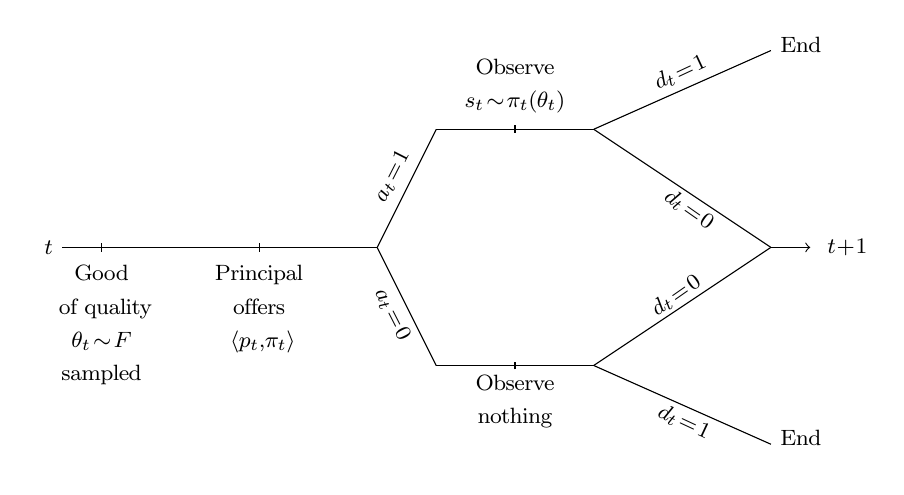
\begin{tikzpicture}[scale=0.5]
\tikzset{
    position label/.style={
             text depth = 1ex
    }
}
    \foreach \x in {-5, -1}
      \draw (\x cm,3pt) -- (\x cm,-3pt);
\draw[-] (-6,0) node[left]{\footnotesize{ $t$}}--(2,0);
\draw[-] (2,0)--(3.5,3);
\draw[-] (2,0)--(3.5,-3);
\draw[-] (3.5,-3)--(7.5,-3);
\draw[-] (3.5,3)--(7.5,3);
\draw[-] (7.5,-3)--(12,0);
\draw[-] (7.5,-3)--(12,-5);
\draw[-] (7.5,3)--(12,5);
\draw[-] (7.5,3)--(12,0);
\draw[->] (12,0)--(13,0)node[right]{\footnotesize{ ${t+1}$}};

\node [position label, align=center, below=3pt] (fend) at (-5,0) {\footnotesize{Good} \\ \footnotesize{ of quality}\\ \footnotesize{$\theta_t\sim F$}\\ \footnotesize{sampled}};
\node [position label, align=center, below=3pt] (fend) at (-1,0) {\footnotesize{Principal} \\ \footnotesize{offers}\\ \footnotesize{ $\langle p_t, \pi_t\rangle$}};
\node [position label, rotate=63, align=center, above] (fend) at (3,1.5) {\footnotesize{$a_t=1$}};
\node [position label, rotate=297, align=center, below] (fend) at (2.8,-1.5) {\footnotesize{$a_t=0$}};


\draw[](5.5,3.1)--(5.5,2.9);
\draw[](5.5,-3.1)--(5.5,-2.9);


\node [position label, align=center, above] (fend) at (5.5,3) {\footnotesize{Observe}\\ \footnotesize{$s_t\sim\pi_t(\theta_t)$}};
\node [position label, align=center, below] (fend) at (5.5,-3) {\footnotesize{Observe}\\ \footnotesize{nothing}};

% \draw[](13,3.1)--(13,2.9);
% \draw[](13,-3.1)--(13,-2.9);
\node [position label, align=center, right] (fend) at (12,5) {\footnotesize{End}};
\node [position label, align=center, right] (fend) at (12,-5) {\footnotesize{End}};

\node [position label, rotate=335, align=center, below] (fend) at (10,-4) {\footnotesize{$d_t=1$}};
\node [position label, rotate=35, align=center, above] (fend) at (10,-1.8) {\footnotesize{$d_t=0$}};

\node [position label, rotate=25, align=center, above] (fend) at (10,3.8) {\footnotesize{$d_t=1$}};
\node [position label, rotate=325, align=center, below] (fend) at (10.2,1.35) {\footnotesize{$d_t=0$}};
  \end{tikzpicture}
  \caption{Timing of events}
  \label{fig:timing}
\end{figure} 

\begin{table}[ht]
\begin{center}
    \begin{tabular}{c|c|c}
         & $a_t=1$& $a_t=0$ \\[8pt] \hline \hline
        $d_t=1$ & $\theta_t-p_t, p_t$& $\theta_t, 0$\\[8pt] \hline
        $d_t=0$& $-p_t, p_t$ & $0,0$
    \end{tabular}
    \caption{Period-$t$ payoffs for the agent and the principal, respectively.}
    \label{tab:payoffs}
    \end{center}
\end{table}

We investigate \textit{stationary} (Perfect Bayesian) equilibrium outcomes of this game, which are  characterized by a strategy specifying contract proposal for the principal, a strategy specifying contract acceptance and search stopping for the agent, and a belief-updating process such that $(i)$  strategies are stationary, i.e.,  history-independent both on and off the equilibrium path, $(ii)$ strategies are sequentially rational, and $(iii)$ beliefs are derived by Bayes rule whenever possible.\footnote{The agent's beliefs are governed by Bayes rule even following an off-path contract proposal by the principal since contracts are proposed without knowledge of the quality of the sampled good. Hence, there are no signaling considerations for the principal.} We provide a more formal definition after we define the contract space. 

\section{Preliminary Analysis}\label{prelim}
\subsection{Signals as posterior-mean distributions}
Suppose the principal proposes a period-$t$ contract $\langle p_t, \pi_t\rangle$ and the agent rejects. The agent's period-$t$ payoff would then be zero if he continues to search whereas his expected payoff would be $m_\varnothing$ if he consumes the good and ends the game. In contrast, if the agent accepts the contract and observes a signal realization $s_t\in S$, he would update his belief about the good's quality from his prior $F$ to a posterior  $F_{s_t}^{\pi_t}$  using Bayes rule. The posterior mean would then be $\mathbb{E}_{F^{\pi_t}_{s_t}}[\theta]$, and the agent's period-$t$ payoff would  be $-p_t$ if he continues to search whereas his expected payoff would be $\mathbb{E}_{F^{\pi_t}_{s_t}}[\theta]-p_t$ if he consumes the good and ends the game. 


Because $\pi_t$ impacts the agent's payoffs only through a good's expected quality, it suffices for our purposes to consider the distribution over posterior means that is induced by the signal. For example, a fully informative signal induces the distribution $F$ while an uninformative signal induces the degenerate distribution $G^\varnothing$ given by
\[
G^\varnothing(m)=\left\{\begin{array}{ccc}
     0 &\mbox{if} & m<m_\varnothing  \\
     1 &\mbox{if} & m\geq m_\varnothing 
     \end{array}\right..
\]

From \cite{bla53} and \cite{rot70}, each signal $\pi$ induces a distribution over posterior means $G^\pi:\Theta\to[0,1]$ that is a mean-preserving contraction of $F$, i.e., %\bph{We could index $G$ in this sentence and in the below display equation with $\pi$, $G^\pi$, to make clearer the dependence. I do not think we need to do it elsewhere}
\[
\int^{\bar \theta}_x G^\pi(m)dm\geq \int^{\bar \theta}_x F(m)dm
\]
for all $x\in\Theta$ with equality at $x=\underline\theta$. 
Conversely, each distribution $G$ that is a  mean-preserving contraction of $F$ can be induced by some signal $\pi$. Thus, without loss of generality, we assume that for each period $t$, the principal can propose a contract of the form $\langle p_t, G_t \rangle \in \mathbb{R}_+\times \mathcal{G}(F)$, where $\mathcal{G}(F)$ is the set of mean-preserving contractions of $F$. Notice that $G^\varnothing$ is a mean-preserving contraction of any $G\in \mathcal{G}(F)$.
\subsection{Signals as convex functions}

Given some posterior-mean distribution $G\in\mathcal{G}(F)$, let $c_G:\Theta\to \mathbb{R}_+$ be defined as
\begin{align*}
 c_G(x)&\triangleq\int^{\bar\theta}_{x}(1-G(m))dm.
\end{align*}
To understand what $c_G(x)$ represents, suppose the agent has a guaranteed payoff of $x\in\Theta$ from some ``outside option." The agent's expected surplus over the outside option from a random draw of distribution $G$ is given by
\begin{align*}
\left(\mathbb{E}_G[m|m\geq x]-x\right)\left(1-G(x)\right)&=\int^{\bar\theta}_x(m-x)dG(m)\\[6pt]
&=c_G(x),
\end{align*}
where the final equality follows from integration by parts.\footnote{The function $c_G$ is often used in characterizing the optimal stopping rule in search models. For example, it is used in \cite{mcc70} to characterize the reservation wage in job search markets, in \cite{wei79} to characterize reservation values when searching over alternatives, and in \cite{wol86} to characterize optimal consumer search behavior. \cite{dog18} refer to $c_G$ as the \textit{incremental-benefit function}.} 

\begin{remark}
\label{remark:1}
For any $G\in\mathcal{G}(F)$, 
\begin{enumerate}[$(a)$]
\item $c_G(\underline\theta)=m_\varnothing-\underline \theta$,
    \item $c_G(\bar\theta)=0$, 
    \item $c_G$ is continuous, weakly decreasing, and  convex, and
    \item $c_G$ is right differentiable with  $\partial_+ c_G(x)=G(x)-1$.
\end{enumerate}

\end{remark}


Intuitively, if the payoff from the outside option is $\underline \theta$, then a random draw from $G$ yields a higher payoff than the outside option with probability one. Thus, $c_G(\underline\theta)=m_\varnothing-\underline\theta$. In contrast, if the payoff from the outside option is $\bar \theta$, then there is zero probability that a random draw from $G$ yields a higher payoff than the outside option. Thus, $c_G(\bar\theta)=0$. Additionally, consider two outside options with payoffs $x$ and $x'$ with $x'>x$; a draw $m$ from $G$ is more likely to exceed $x$ than $x'$, and even if $m$ exceeds both, $m-x>m-x'$. These two properties combined imply that $c_G(x)$ is a weakly decreasing and convex function of $x$. Convexity further implies that $c_G(x)$ is left- and right-differentiable for all $x\in\Theta$. It suffices to consider only the right derivative for our purposes.\footnote{Both the left and right derivatives of $c_G$ are well-defined as $G$ is c\`adl\`ag. The left derivative is given by $\partial_-c_G(x)=G(x_-)-1$. $c_G$ is differentiable everywhere but at the mass points of $G$.}

Notice that if $G'$ is a mean-preserving contraction of $G''$, then $c_{G'}\leq c_{G''}$ pointwise. Hence, for all $G\in\mathcal{G}(F)$,  $c_{G^\varnothing}\leq c_G\leq c_F$ pointwise. Let $\mathcal{C}(F)$ be the set of continuous, weakly decreasing, and convex functions $c:\Theta\to \mathbb{R}_+$ such that $c_{G^\varnothing}\leq c\leq c_F$ pointwise. Then for all $G\in\mathcal{G}(F)$, $c_G\in\mathcal{C}(F)$. Additionally, for each $c\in\mathcal{C}(F)$, there exists a distribution $G\in \mathcal{G}(F)$ such that $c=c_G$  (Proposition 1, \cite{gen16}). Therefore, we can represent signals not only as distributions in $\mathcal{G}(F)$ but also as functions in $\mathcal{C}(F)$.

\subsection{Agent's search problem}\label{autarky_section}
Before we analyze the principal-agent game, we first consider a hypothetical setting in which there is no principal, and the agent  observes a realization from some signal $G\in \mathcal{G}(F)$ for free in each period. This setting is instructive in characterizing when there is scope in our main model for contracting between the principal and the agent.  

Let $u(G)$ be the agent's ex-ante payoff in this search problem, which in a stationary setting is also his continuation payoff. The agent  searches until he finds a good  whose expected quality exceeds his discounted continuation value $\delta u(G)$. Thus, the agent's payoff $u(G)$ is the unique solution to the fixed point (as a function of $u$)
\begin{align*}
 \label{eq:1}
\tag{1}
 u&=\int_\Theta \max\{m, \delta u\}dG(m).
\end{align*}
% \begin{align*}
%  \label{eq:1}
% \tag{1}
%  u&=\underbrace{\delta u}_{\substack{\text{Reservation}\\\text{value}}}+\underbrace{\int_\Theta \max\{m-\delta u, 0\}dG(m)}_{\substack{\text{Expected surplus}\\ \text{from search}}}.
% \end{align*}

As the integrand is a convex function of $m$, the agent benefits from a ``more dispersed" distribution of posterior means. Formally, $u(G')\leq u(G'')$ whenever $G'$ is a mean-preserving contraction of $G''$. Thus, the highest surplus that can be generated in the search market is $\bar u\triangleq u(F)>0$ while the lowest surplus that can be generated is $\underline u\triangleq u(G^\varnothing)=\max\{m_\varnothing, 0\}$. We refer to $\bar u$ as the socially efficient surplus and to $\underline u$ as the agent's autarky payoff.


If $\underline u=\bar u$, we say the agent \textit{never searches} because  it would be optimal in this case for the agent to stop searching and consume the first good he samples after observing any realization from any $G\in\mathcal{G}(F)$. Intuitively, an agent never searches when the lowest quality good yields a sufficiently high payoff; even if the agent knew he would sample a good of quality $\bar \theta$ in the next period, he would prefer to accept a good of quality $\underline \theta$ today. \autoref{lemma:1} presents a sufficient and necessary condition for when the agent never searches.



\begin{lemma}
\label{lemma:1}
The agent never searches if and only if $\underline \theta\geq \delta m_\varnothing$. 
\end{lemma}

The above lemma implies that if $\underline \theta\geq \delta m_\varnothing$, the agent would have no value for information, making the contracting game between the agent and the principal trivial. We therefore make the following assumption hereafter:

\begin{assumption}\label{ass:1}
$\underline \theta<\delta m_\varnothing$.
\end{assumption}

\hyperref[ass:1]{\Cref{ass:1}} is satisfied for all $\delta \in(0,1)$ if $\underline \theta\leq  0$. However, if $\underline \theta> 0$, the assumption places further restrictions on the values of the discount factor. The assumption allows us to rewrite the fixed-point problem in \eqref{eq:1} as
\begin{align*}
    u&=\delta u \int_{\underline \theta}^{\delta u}dG(m)+\int_{\delta u}^{\bar\theta}mdG(m)\\[6pt]
    &=\delta u+\int^{\bar\theta}_{\delta u}(m-\delta u)dG(m)\\[6pt]
    \label{eq:1'}
    \tag{$1'$}
    &=\underbrace{\delta u}_{\substack{\text{reservation}\\\text{value}}} + \underbrace{c_G(\delta u)}_{\substack{\text{added value}\\\text{from search}}}
\end{align*}

\noindent where the final equality follows because \hyperref[ass:1]{\Cref{ass:1}} implies $\delta u(G)\in(\underline \theta, \bar \theta)$ for any $G\in \mathcal{G}(F)$, i.e. that $c_G(\delta u)$ is well defined.

Let $r(G)\triangleq \delta u(G)$ denote the agent's reservation value. We can re-purpose \eqref{eq:1'} so as to characterize $r(G)$ as the unique solution to the fixed point  (as a function of $r$)
\begin{align*}
 r&=\delta\big( r+c_G(r)\big)\\[6pt]
 \label{eq:2}
 \tag{2}
 &=\left(\frac{\delta}{1-\delta}\right)\cdot c_G(r).
\end{align*}
 The fixed point in \eqref{eq:2} is particularly amenable to a geometric representation as shown in \autoref{fig:fix}. Since $c_{G'}\leq c_{G''}$ pointwise whenever $G'$ is a mean-preserving contraction of $G''$, the highest reservation value is $\bar r\triangleq r(F)$ and the lowest reservation value is $\underline r\triangleq r(G^\varnothing)$. We refer to $\bar r$ as the efficient reservation value and to $\underline r$ as the autarky reservation value. 


\begin{figure}[ht]
\begin{center}
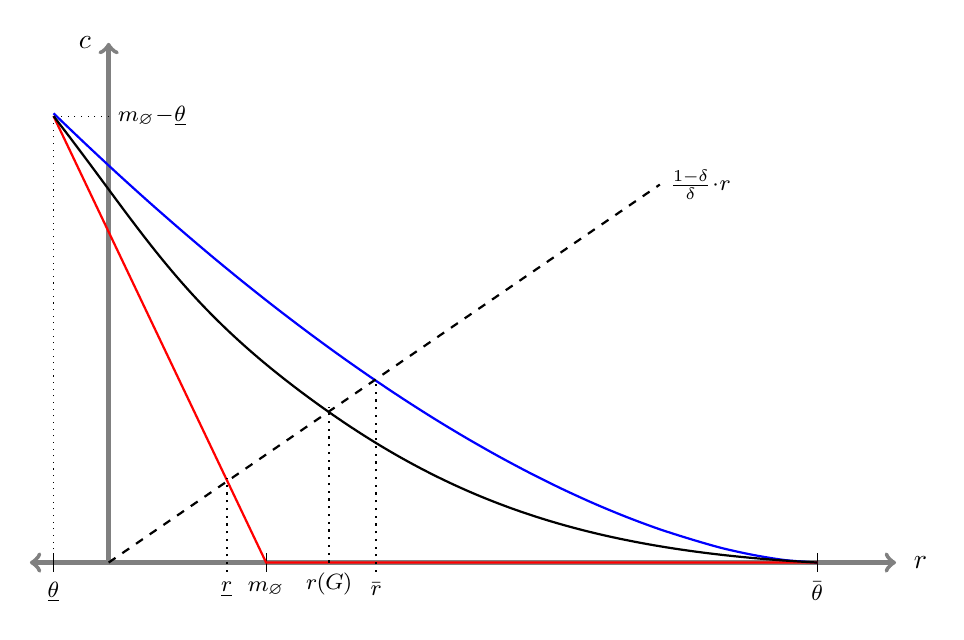
\begin{tikzpicture}[xscale=10, yscale=6]
% axis lines and labels
\draw [<->, help lines, ultra thick] (0,0) -- (1.1,0);
\draw [->, help lines, ultra thick] (0.1,0) --(.1,1.1);\node[right=3pt] at (1.1,0) {$r$};
\node[left=3pt] at (0.1, 1.1) {$c$};

% Support of F
\draw [] (1,-.02)node[below]{\footnotesize{$\bar\theta$}}--(1,.02);
\draw [] (.03,-.02) node[below]{\footnotesize{$\underline\theta$}}--(.03,.02);
\draw [dotted] (0.1, .945)node[right]{\footnotesize{$m_\varnothing -\underline\theta$}}--(0.03,.945);
\draw [dotted] (.03, 0)--(.03,.945);
\draw [] (.3,-.02) node[below]{\footnotesize{$m_\varnothing$}}--(.3,.02);

%curves
\draw[blue, domain=0.03:1,smooth,variable=\x, thick] plot ({\x},{(1-\x)^1.65});
\draw[thick, red](.03, .945)--(.3,0)--(1,0);
\draw[ thick] plot [smooth, tension=2] (0.03,.945)to [in=130, out=295](.37, .33) to [in=175, out=310](1,0);

%fixed point operator
\draw[thick, dashed] (0.1,0)--(.8,.8)node[right]{\footnotesize{$\frac{1-\delta}{\delta}\cdot r$}};

% fixed points
\draw [dotted, thick] (.38,0) node[below]{\footnotesize{$r(G)$}}--(.38,.33);
\draw [dotted, thick] (.25,-.02) node[below]{\footnotesize{$\underline r$}}--(.25,.18);
\draw [dotted, thick] (.44,-.02) node[below]{\footnotesize{$\bar r$}}--(.44,.39);
\end{tikzpicture}
\caption{Example with $\underline \theta<0<m_\varnothing<\bar \theta$. The dashed line has a slope of $(1-\delta)/\delta$. The red curve is $c_{G^\varnothing}$, the black curve is $c_G$ for some arbitrary $G\in\mathcal{G}(F)$, and the blue curve is $c_F$. The intersection of each respective curve with the dashed line represents the solution to the fixed point problem in \eqref{eq:2}.}
\label{fig:fix}
\end{center}
\end{figure}

\section{Stationary Equilibrium}\label{stationary}
In this section, we characterize stationary equilibrium outcomes. To that end, we first make two observations that simplify our task. First,  it suffices for our purposes to consider only pure strategies because, since all players are risk neutral and the space of contracts is convex, the principal does not gain from randomizing over contracts.\footnote{Additionally, to sustain an equilibrium, we also assume that whenever the agent is indifferent between any two actions on the equilibrium path, he chooses the one that maximizes the principal's payoff.} Second,  we can restrict attention to contracts that induce the agent to accept since the agent rejecting a contract is payoff-equivalent for all players to the accepting a contract $\langle 0, G^\varnothing\rangle$.

\begin{definition}
\label{def:1}
\normalfont A stationary equilibrium is defined by a pair of agent-principal continuation values $(U, V)\in \mathbb{R}^2$ and a contract $\langle p,G\rangle\in\mathbb{R}_+\times \mathcal{G}(F)$ such that in each period and after every history:
\begin{enumerate}
    \item The agent stops searching and consumes a good of expected quality $m\in\Theta$ if and only if \footnote{When $m=\delta U$, the agent is indifferent between stopping and continuing his search while the principal (weakly) prefers for the agent to continue his search. In \autoref{prop:1}, we show that the equilibrium signal never leaves the agent indifferent between stopping and searching.}  
    \[
     \label{eq:os}
    \tag{OS}
    m>\delta U,
    \]
    \item The agent accepts a contract $\langle \widehat p,\widehat G\rangle\in\mathbb{R}_+\times\mathcal{G}(F)$  if and only if
    \begin{align*}
        \underbrace{\delta U+c_{\widehat G}(\delta U)-\widehat p}_{\text{payoff from accept}}&\geq \underbrace{\delta U+c_{ G^\varnothing}(\delta U)}_{\text{payoff from reject}} \\[8pt]
        \label{eq:pc}
    \tag{PC}
        \Leftrightarrow   c_{\widehat G}(\delta U)-c_{G^\varnothing}(\delta U)& \geq \widehat p,
    \end{align*}
       
\item The principal proposes contract $\langle p,G\rangle$ to maximize her profit, i.e.,
\[
\label{eq:pm}
\tag{PM}
 \langle p,G\rangle\in \argmax_{\langle \widehat p, \widehat G\rangle\in\mathbb{R}_+\times \mathcal{G}(F)}\hspace*{.2em} \widehat p+ \widehat G(\delta U) \delta V \hspace*{.5em} \text{ subject to \eqref{eq:pc}},
\]   
\item Payoffs are self-generating, i.e., 
\[
\label{eq:sga}
\tag{SG-A}
U=\delta U+c_{G}(\delta U)-p 
\] 
    and
    \[
    \label{eq:sgp}
\tag{SG-P}
V= p + G(\delta U) \delta V.
\] 
\end{enumerate}
\end{definition}

In words, in a stationary equilibrium, the agent and the principal anticipate the continuation values $U$ and $V$ in each period following any history of events. The agent then optimally stops searching whenever he samples a good with expected quality that exceeds his discounted continuation value $\delta U$. This optimal stopping rule is captured by \eqref{eq:os}. Additionally, the agent optimally accepts any contract that gives him a higher payoff than $\delta U+c_{G^\varnothing}(\delta U)=\max\{m_\varnothing, \delta U\}$, which is the payoff he  gets  by either consuming the good in the current period without observing a signal or by waiting for the next period. The constraint \eqref{eq:pc} captures the agent's contract acceptance decision. \eqref{eq:os} and \eqref{eq:pc} together imply that the agent is sequentially rational following any contract proposal by the principal. 

 Given the anticipated continuation values and the agent's strategies, the principal then proposes a contract that maximizes the sum of her per-period revenue $\widehat{p}$ and her expected discounted continuation value $\widehat G(\delta U)\delta V$. We formulate the principal's contract proposal as a constrained maximization problem in \eqref{eq:pm}. Finally, the anticipated continuation values must be consistent with the agent's and principal's stationary equilibrium strategies, which is captured by \eqref{eq:sga} and \eqref{eq:sgp}. 

 
To gain some intuition of the economic forces at play, it is instructive to separate the \textit{intra-temporal trade-offs}\textemdash trade-offs the principal faces when proposing a contract in the current period while  holding contracts in subsequent periods fixed\textemdash from the \textit{inter-temporal trade-offs}\textemdash the trade-offs the principal faces when considering different future contracts.  

Let us first consider the intra-temporal trade-offs in some period $t\geq 1$. Suppose the principal proposes the contract $\langle \widehat p,\widehat G\rangle$ in period $t$ and proposes $\langle p, G\rangle$ thereafter. From \eqref{eq:sga} and \eqref{eq:sgp}, we can compute the continuation values $U$ and $V$ associated with the principal proposing the contract $\langle p, G\rangle$ in all subsequent periods. Holding the  pair $(U, V)$ fixed, the period-$t$ contract $\langle \widehat p,\widehat G\rangle$ impacts the agent's search problem along an intensive and extensive margin. For the intensive margin, conditional on the agent accepting the contract, $\langle \widehat p, \widehat G\rangle$ impacts the probability that the agent discontinues search in period $t$, which is given by $1-\widehat G(\delta U)$. For the extensive margin, the contract $\langle \widehat p,\widehat G\rangle$ affects whether the agent even purchases a signal from the principal. This impact on the extensive margin is captured by the participation constraint \eqref{eq:pc}. 
 

% If the profit-maximizing period-$t$ contract is $(p, G)$, then we have in fact found a stationary equilibrium. 

Next, let us consider the inter-temporal  trade-offs. Suppose the principal instead considers proposing a contract $\langle p', G\rangle$ in period $t+1$ and onward with $p'>p$. From \eqref{eq:sga} and \eqref{eq:sgp}, assuming the agent accepts the new contract, we can compute the associated continuation values $U'$ and $V'$. A higher price $p'$ has a direct positive effect on the principal's continuation payoff $V'$.  However, a higher price also has a  direct negative effect on the agent's continuation value $U'$, which consequently also affects \eqref{eq:os} by lowering the optimal stopping threshold; thus, an increase in $p'$ has an indirect negative effect on the principal's continuation value by decreasing the expected length of time the agent remains in the search market. The principal must trade-off having high prices and a short contractual relationship with the agent against having low prices and a long contractual relationship. A similar, albeit less transparent, trade-off exists when changing the signal. For example, proposing a contract $\langle p, G'\rangle$ instead of $\langle p, G \rangle$ in period $t+1$ and onward could change the agent's continuation value from $U$ to $U'$ when $G$ and $G'$ differ in their informativeness. When the same contract optimizes both the intra- and inter-temporal trade-offs, then we have in fact found a stationary equilibrium.

In order to state our main result, we first introduce a ``pass/fail" signal where $S=\{\text{fail, pass}\}$ and 
 \[
\pi(\text{pass}|\theta)=\left\{\begin{array}{ccl}
     0 &\mbox{if} & ~~~\theta\leq  \bar   r \\
     1 &\mbox{if} & ~~~\theta> \bar r
     \end{array}\right.,
\] 
which induces a binary distribution $G^*\in\mathcal{G}(F)$ given by 
 \[
 \label{eq:3}
\tag{3}
G^*(m)=\left\{\begin{array}{ccl}
     0 &\mbox{if} & ~~~m<\mathbb{E}_F[\theta|\theta\leq  \bar   r]  \\
       F( \bar r) &\mbox{if} &~~~ \mathbb{E}_F[\theta|\theta\leq  \bar r]\leq m<\mathbb{E}_F[\theta|\theta>  \bar r]  \\
     1 &\mbox{if} & ~~~m\geq \mathbb{E}_F[\theta|\theta>  \bar   r]
     \end{array}\right..
\]
We call this distribution binary as it has mass at only two values, namely $\mathbb{E}_F[\theta|\theta\leq  \bar r]$ and $\mathbb{E}_F[\theta|\theta>  \bar r]$. As this distribution is useful in characterizing stationary equilibria, we state some of its properties in the following lemma, which are graphically summarized in \autoref{fig:1.optimal_pass_fail}.

\begin{lemma}\ 
\label{lemma:2}
\begin{enumerate}[$(i)$]
\item $c_{G^*}(x)\leq c_F(x)$ for all $x\in\Theta$ with a point of tangency at $x=\bar r$. 
\item $r(G^*)=r(F)$.
\item  $r(G)<r(G^*)$ for all binary distributions $G\in\mathcal{G}(F)$ with $G\neq G^*$.
\item $G^*(m)=F(\bar r)$ for all $m\in [\underline r, \bar r]$. 
\end{enumerate}
\end{lemma}\

\begin{figure}[ht]
\begin{center}
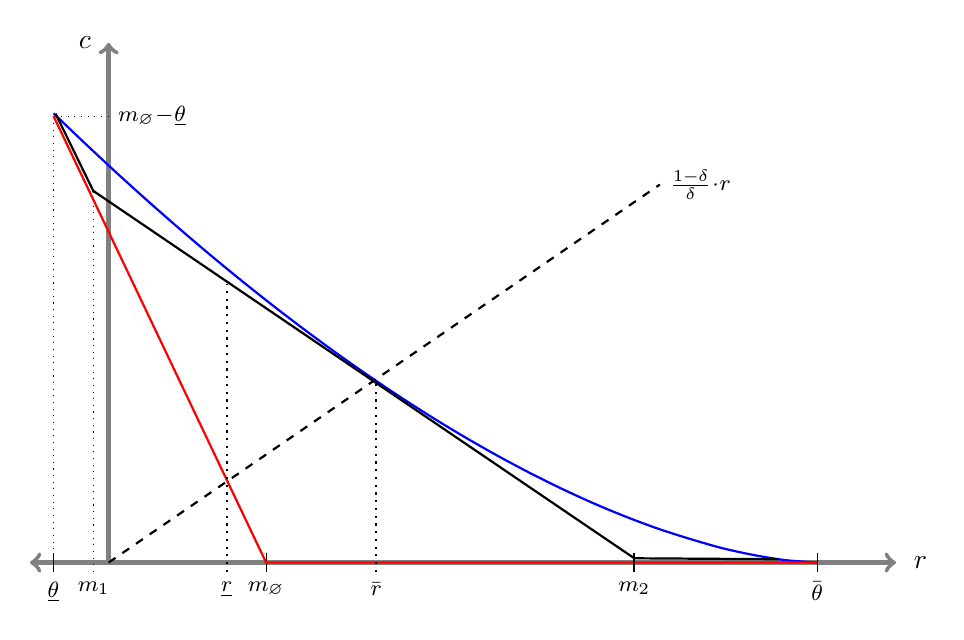
\begin{tikzpicture}[xscale=10, yscale=6]
% axis lines and labels
\draw [<->, help lines, ultra thick] (0,0) -- (1.1,0);
\draw [->, help lines, ultra thick] (0.1,0) --(.1,1.1);\node[right=3pt] at (1.1,0) {$r$};
\node[left=3pt] at (0.1, 1.1) {$c$};

% Support of F
\draw [] (1,-.02)node[below]{\footnotesize{$\bar\theta$}}--(1,.02);
\draw [] (.03,-.02) node[below]{\footnotesize{$\underline\theta$}}--(.03,.02);
\draw [dotted] (0.1, .945)node[right]{\footnotesize{$m_\varnothing -\underline\theta$}}--(0.03,.945);
\draw [dotted] (.03, 0)--(.03,.945);
\draw [] (.3,-.02) node[below]{\footnotesize{$m_\varnothing$}}--(.3,.02);

%curves
\draw[blue, domain=0.03:1,smooth,variable=\x, thick] plot ({\x},{(1-\x)^1.65});
\draw[thick, red](.03, .945)--(.3,0)--(1,0);
%\draw[ thick](.0327, .95)--(.18,.435)--(.55,.38)--(.75,.009);
\draw[domain=0.0799:.768,smooth,variable=\x, thick] plot ({\x},{-1.131895*(\x-.44)+.3798});
\draw[ thick](.0327, .95)--(.0813,.784);
\draw[ thick](.7675,.009)--(.95,.007);

%support of G^*
\draw[dotted](.0813,-0.02)node[below]{\footnotesize{$m_1$}}--(.0813,.784);
\draw[ thick](.7675,-0.02)node[below]{\footnotesize{$m_2$}}--(.7675,0.02);
%fixed point operator
\draw[thick, dashed] (0.1,0)--(.8,.8)node[right]{\footnotesize{$\frac{1-\delta}{\delta}\cdot r$}};

% fixed points
\draw [dotted, thick] (.25,-.02) node[below]{\footnotesize{$\underline r$}}--(.25,.59);
\draw [dotted, thick] (.44,-.02) node[below]{\footnotesize{$\bar r$}}--(.44,.39);

% %price
% \draw [decorate,decoration={brace,amplitude=10pt}]
% (0.255,0.583) -- (0.255,.185) node [black,midway,xshift=0.6cm]
% {\footnotesize $p$};

\end{tikzpicture}
\caption{The red curve is $c_{G^\varnothing}$, the black curve is $c_{G^*}$, the blue curve is $c_F$, and  $m_1\triangleq\mathbb{E}_F[\theta|\theta\leq \bar r]$ and $m_2\triangleq\mathbb{E}_F[\theta|\theta> \bar r]$. Note that $c_{G^*}$ is tangent to $c_F$ at $\bar r$. }
\label{fig:1.optimal_pass_fail}
\end{center}
\end{figure}


% Second, $c_F(x)\geq c_{G^*}(x)$ for all $x\in\Theta$ with a point of tangency at $x=\bar r$ as shown in \autoref{fig:1.optimal_pass_fail} \bph{I think we should add an explanation for this tangency point. 1) $c_F(x)\geq c_{G^*}(x)$ for all $x\in\Theta$ because $F$ is Blackwell more informative than every $G\in \mathcal{G}(F)$, and in particular, than $G^*$. 2) $\bar{r}\in(\underline \theta,\bar\theta)$ which we discuss is an implication of Assumption 1 just before \eqref{eq:2}. Therefore, by full support of $F$ it follows that $m_1:=\mathbb{E}_F[\theta|\theta\leq  \bar r]<\bar r< \mathbb{E}_F[\theta|\theta>  \bar r].$ 3) Point 2), \eqref{eq:3}, and the definition of $c_G$ on page 5 (which isn't a display equation we can cross reference as of now, but we could change) imply that  $c_F(\bar r)=c_{G^*}(\bar r)$. 4) This one is about the point of tangency, and I'll reference the properties in the bulleted list on page 6:  (i) $c_F(x)> c_{G^\varnothing}(x)=c_{G^*}(x)$ for all $x\in(\underline\theta,m_1].$ The inequality follows because $m_1=\mathbb{E}_F[\theta|\theta\leq  \bar r]<\mathbb{E}_F[\theta]=m_\varnothing$ by construction and  point (d) on page 6 implies $\partial_+ c_{G^\varnothing}(x)=-1$ for all $x<m_\varnothing$ and $\partial_+ c_{F}(x)=F(x)-1>-1$ for all $x\in(\underline\theta,\bar{\theta}$ since $F(x)>0$ for all $x>\underline\theta.$ Point (d) also reveals that $c_{G^\varnothing}(x)=c_{G^*}(x)$ for $x<\min\{m_1,m_\varnothing\}=m_1$. (ii) Point (d) on page 6 also implies that $c_F$ is strictly convex and strictly decreasing, while \eqref{eq:3} implies that $c_G(x)$ is linear for $x\in[m_1,m_2).$ (iii) Combining the above: $c_{G^*}(m_1)<c_{F}(m_1)$ and $c_{G^*}(\bar r)=c_{F}(\bar r)$ implies that $c_F$ and $c_{G^*}$ are tangent at $\bar r$, since $c_{F}$ is strictly convex and strictly decreasing, $c_{G^*}$ is linear and strictly decreasing on $[m_1,m_2)$, and since $c_F(x)\geq c_{G^*}(x)$ for all $x\in[\underline \theta,\bar \theta]$ for all $G\in\mathcal{G}(F),$...\textbf{perhaps this could be rolled in with the other properties discussed later in the paragraph into a formal lemma   }}. We can then show that, by \eqref{eq:2}, $r(G^*)=r(F)\triangleq\bar r$. In other words, $G^*$ yields the efficient reservation value and is in fact the unique binary posterior-mean distribution that can do so. Finally,  given \hyperref[ass:1]{Assumption 1}, $G^*(m)\in(0,1)$ and constant for $m\in [\underline r, \bar r]$. We provide a more detailed discussion of these properties in the \hyperref[appendix]{Appendix}. \bph{as stated during our discussion yesterday, I think these points should be packaged into a lemma/remark/whatever here. Then the proof should be in appendix.}

Our main result, \autoref{prop:1} below, establishes not only the existence of a stationary equilibrium but also that all stationary equilibria are payoff equivalent. In any stationary equilibrium, the socially efficient surplus $\bar u$ is generated but the agent's payoff is the same as his autarky payoff $\underline u$. The remaining surplus $\bar u-\underline u$ is extracted by the principal. 

Given that the agent earns his autarky payoff, he would be willing to stop searching whenever the expected quality of a sampled good exceeds the autarky reservation value $\underline r$. However, in equilibrium, the agent does not stop searching until he samples a good whose quality exceeds the efficient threshold $\bar r$.\footnote{Under \hyperref[ass:1]{Assumption 1}, $\underline \theta<\underline r<\bar r<\bar\theta$.} In other words, the agent searches as if he observes a fully informative signal  for free, even though his payoff is as if he observes no information.

In order to induce this seemingly contradictory behavior in the agent, the principal offers a contract in which the signal pools sufficiently high quality goods\textemdash for which the agent would be willing to stop his search\textemdash with sufficiently low quality goods\textemdash for which the agent would rather continue searching. One example is the pass/fail signal  that generates the distribution  $G^*$ in \eqref{eq:3}. This signal pools and labels all goods of quality less than $\bar r$ as a ``fail" and all other goods as a ``pass."  Importantly, the agent is unable to distinguish between a good whose quality lies in the interval $[\underline r, \bar r]$ from a good whose quality is lower than $\underline r$. We can see in \autoref{fig:1.optimal_pass_fail} that $\mathbb{E}_F[\theta|\theta\leq \bar r]=m_1<\underline r$, and the proof of part $(iv)$ of \autoref{lemma:2} shows that this property holds more generally for any prior $F$. Therefore, whenever the agent sees a ``fail," he is persuaded to continue searching. 

The principal then sets the price $p$ of such a pooling signal to equal the value of information generated in a single period. Interestingly, $p$ is a (possibly small) fraction of the maximal net surplus $\bar u-\underline u$ that the principal ultimately extracts.\footnote{As we show in point $(iii)$ of \autoref{prop:1}, the per-period price is strictly below $\bar u-\underline u$ for any $\delta>0$. Additionally, as $\delta\to 1$, the per-period price converges to zero while the duration of search goes to infinity. } However, the principal is able to persuade the agent to search for longer than he otherwise would like, allowing the principal to extract the maximal net surplus through dribs and drabs.
\newline 
\begin{theorem}\label{prop:1}\
A stationary equilibrium exists. A pair of agent-principal continuation values $(U, V)\in \mathbb{R}^2$ and a contract $\langle p,G\rangle\in\mathbb{R}_+\times \mathcal{G}(F)$ constitute a stationary equilibrium if and only if
\begin{enumerate}[$(i)$]
    \item  $U=\underline u$, 
    \item  $V=\bar u-\underline u$, 
        \item  $p=(\bar u-\underline u)\big(1-\delta F( \bar r)\big)$,
    \item $G(\underline r)=F( \bar r)$, and
    \item $c_G(x)\geq c_{G^*}(x)$ for all $x\in\Theta$ with equality at $x=\underline r$.
\end{enumerate}
\end{theorem}




% In order to achieve this seemingly contradictory behavior in the agent, the principal proposes a contract in which the per-period price $p$ is a (possibly very small) fraction of the extracted surplus. The low price keeps the agent's continuation value high enough that he does not end his search too early. Additionally, the principal proposes a contract in which the signal structure, for example, pools all goods  whose quality is lower than $\bar r$ and labels them as ``fail."  This persuades the agent to continue searching whenever he sees a signal realization of ``fail"  because he is unable to distinguish the goods whose quality lies in the interval $[\underline r, \bar r]$\textemdash goods for which the agent would be willing to stop his search\textemdash from the goods whose quality is lower than $\underline r$\textemdash goods for which the agent would rather continue searching. The price and the signal structure combined persuade the agent  to search for longer than he otherwise would like, allowing the principal to extract the surplus through dribs and drabs.


\noindent\begin{proof} 
% We first show the ``only if" direction by arguing that any stationary equilibrium must satisfy $(i)-(v)$ of \autoref{prop:1}. 

\noindent ($\Rightarrow$) Suppose a contract $\langle p, G\rangle $ along with a pair of agent-principal continuation values $(U, V)$ constitute a stationary equilibrium. Then the contract $\langle p,G\rangle$ must be consistent with the fixed-point problem given in \eqref{eq:sga}. Additionally, from \eqref{eq:pm} and \eqref{eq:sgp},  $\langle p,G\rangle$ also solves the maximization problem 
\[
\label{eq:4}
\tag{4}
V=\max_{\langle \widehat p,\widehat G \rangle\in\mathbb{R}_+\times \mathcal{G}(F)} \hspace*{.3em}\frac{\widehat p}{1-\delta \widehat G(\delta U)}\hspace*{.5em} \text{ subject to \eqref{eq:pc}}.
\]

Since the objective function in \eqref{eq:4} is increasing in the price $\hat p$, the constraint \eqref{eq:pc} must   bind at the maximum, i.e., $p=c_{G}(\delta U)-c_{G^\varnothing}(\delta U)$. The fixed-point problem in \eqref{eq:sga} then becomes  
\[
U=\delta U+c_{G^\varnothing}(\delta U),
\]
which, by evaluating \eqref{eq:1'} at $G^\varnothing$, has a unique solution $U=u(G^\varnothing)\triangleq \underline u$  establishing point $(i)$ of the theorem.

From \eqref{eq:os}, the agent's optimal stopping rule is characterized by the autarky reservation value $\delta\underline u\triangleq \underline r$. The maximization problem in \eqref{eq:4} can now be written as  
\[
\label{eq:44}
\tag{$4'$}
V=\max_{\widehat G\in\mathcal{G}(F)} \hspace*{.3em}\frac{c_{\widehat G}( \underline r)-c_{G^\varnothing}(\underline r)}{1-\delta \widehat G( \underline r)}.
\]
By \hyperref[ass:1]{Assumption 1}, the objective function in \eqref{eq:44} is strictly positive when evaluated at $\widehat G=F$. Thus,  $V>0$. 

Since $\langle p, G\rangle$ is a solution to \eqref{eq:4}, $G$ is a solution to \eqref{eq:44}. Additionally, the agent must  both stop and continue his search in each period with a positive probability, i.e., $G(\underline r)\in (0,1)$.
% Otherwise, the distribution $G$ would induce the agent to either always stop or to never stop his search regardless of the realized posterior mean. There would be no value of information associated with such a distribution and the agent would not be willing to buy it from the principal for a positive price. Thus, the principal's profit from inducing a distribution with $G(\underline r)=0$ or $G(\underline r)=1$ would be zero, which contradicts our earlier statement that $V>0$.
\footnote{The proof is as follows: suppose for contradiction that $G(\underline r)=0$, then 
\begin{align*}
    c_G(\underline r)&=c_G(\underline \theta)-\int_{\underline \theta}^{\underline r}\big(1-G(m)\big)dm \leq c_{G^\varnothing}(\underline \theta)-\int_{\underline \theta}^{\underline r}\big(1-G_{\varnothing}(m)\big)dm =c_{G^\varnothing}(\underline r),
\end{align*}
where the inequality follows because $c_G(\underline \theta)=c_{G^\varnothing}(\underline \theta)$ by point $(a)$ of  \autoref{remark:1} and because $0=G(m)\leq G_{\varnothing}(m)$ for all $m\leq \underline r$. If instead $G(\underline r)=1$, then 
\[
c_G(\underline r)=\int^{\bar\theta}_{\underline r}\big(1-G(m)\big)dm\leq \int^{\bar\theta}_{\underline r}\big(1-G^\varnothing(m)\big)dm=c_{G^\varnothing}(\underline r), 
\]
where the inequality follows from the fact that $0=1-G(m)\leq 1-G_{\varnothing}(m)$ for all $m\geq \underline r$. 

In either case, since $G^\varnothing$ is a mean-preserving contraction of $G$, we have $c_G\geq c_{G^\varnothing}$ pointwise, which implies that $c_G(\underline r)=c_{G^\varnothing}(\underline r)$. Consequently, the solution to \eqref{eq:44} would be  $V=0$, which establishes a contradiction. } 

From the distribution $G$, we derive a binary distribution $G^\dagger\in \mathcal{G}(F)$ given by 
% \bph{here's a purely notational comment: we could swap $G^*$ and $G^\dagger$ for $\bar G$ and $\underline G$, respectively. This would then tie the location of the bar to comport with the bar in the $r$ term in the conditional expectation EDIT: ah, this is actually more complicated than I thought, because $G^\dagger$ depends on $G$, so if we want to change the index it would make sense to index it by $G$ (but then of course, that would be frustrating notation since we use $G$ as an arbitrary distribution but also our equilibrium one. Maybe we can talk in person}
\[
G^\dagger(m)=\left\{\begin{array}{ccl}
     0 &\mbox{if} &~~~ m<\mathbb{E}_{ G}[\theta|\theta\leq  \underline   r]  \\
        G(\underline r) &\mbox{if} &~~~ \mathbb{E}_{ G}[\theta|\theta\leq \underline r]\leq m<\mathbb{E}_{ G}[\theta|\theta> \underline r]  \\
     1 &\mbox{if} &~~~ m\geq \mathbb{E}_{ G}[\theta|\theta>  \underline r]
     \end{array}\right..
\]
The terms $\mathbb{E}_{ G}[\theta|\theta\leq  \underline   r]$ and $\mathbb{E}_{ G}[\theta|\theta>  \underline r]$ exist as $G(\underline r)\in (0,1)$, so $G^\dagger$ is well-defined.
\begin{remark}\
\label{remark:2}
    \begin{enumerate}[$(a)$]
        \item By construction, $\mathbb{E}_{ G}[\theta|\theta\leq  \underline   r]<\underline r<\mathbb{E}_{ G}[\theta|\theta>  \underline   r]$. Thus, $G^\dagger(\underline r)=G(\underline r)$.
        \item $G^\dagger$ is a mean-preserving contraction of $G$. Hence,  $c_{G^\dagger}(x)\leq c_{G}(x)$ for all $x\in\Theta$.\footnote{Note that $G^\dagger$ is derived as  a function of only $G$ and thus cannot be more informative. It is also possible to directly verify $c_{G^\dagger}\leq c_G$ pointwise.} Additionally, 
        \begin{align*}
    c_G(\underline r)&=\int_{\underline r}^{\bar \theta}(m-\underline r)dG(m)\\[6pt]
    &=\big(\mathbb{E}_{G}[\theta|\theta\geq \underline r]-\underline r\big)\big(1-G(\underline r)\big)\\[6pt]
    &=\big(\mathbb{E}_{G}[\theta|\theta\geq \underline r]-\underline r\big)\big(1-G^\dagger(\underline r)\big)\\[6pt]
&=c_{G^\dagger}(\underline r).
\end{align*}
\end{enumerate}
\end{remark}\vspace*{1em} 

\noindent We apply \autoref{remark:2} to \eqref{eq:44}, which yields
\[
\frac{c_{ G^\dagger}(\underline r)-c_{G^\varnothing}(\underline r)}{1-\delta  G^\dagger(\underline r)}=\frac{c_{ G}(\underline r)-c_{G^\varnothing}(\underline r)}{1-\delta  G(\underline r)}.
\]
Thus, $G^\dagger$ is also a solution to \eqref{eq:44}. In fact, for any binary distribution $\widehat G\in\mathcal{G}(F)$ with $\widehat G(\underline r)\in (0,1)$, we have 
\begin{align*}
    V&=\frac{c_{ G^\dagger}(\underline r)-c_{G^\varnothing}(\underline r)}{1-\delta  G^\dagger(\underline r)}\\[9pt]
    &\geq \frac{c_{ \widehat G}(\underline r)-c_{G^\varnothing}(\underline r)}{1-\delta  \widehat G(\underline r)}\\[9pt]
    &= \frac{c_{ \widehat G}(r(\widehat G))+\displaystyle\int_{ \underline r}^{r(\widehat G)}(1-\widehat G(m))dm -c_{G^\varnothing}(\underline r)}{1-\delta  \widehat G( \underline r)}\\[9pt]
    &=\frac{\big(r(\widehat G)-\underline r\big)\left(\frac{1-\delta}{\delta}\right)+\big(r(\widehat G)-\underline r\big)\big(1-\widehat G(\underline r)\big)}{1-\delta  \widehat G(\underline r)}\\[9pt]
    &=\frac{r(\widehat G)-\underline r}{\delta},
\end{align*}
where the inequality follows because $G^\dagger$ solves \eqref{eq:44} with equality, the second equality follows from breaking up the limits of the integral in $c_{\widehat G}(\underline r)$, the first term in the numerator of the third equality follows from $r(G')$ being the unique reservation value that solves \eqref{eq:2} computed for $G'=\widehat G$ and $G'=G^\varnothing$, and the second term in the numerator of the third equality follows by the fact that a binary distribution $\widehat G$ with $\widehat G(\underline r)\in (0,1)$ must be constant over the interval $[\underline r, r(\widehat G)]$.

 However, by \autoref{lemma:2}, the distribution $G^*$ defined in \eqref{eq:3} is the unique binary distribution that simultaneously satisfies $G^*(\underline r)\in(0,1)$ and $r(G^*)=\bar r$. Hence,  $r(G^*)> r(\widehat G)$ for all other binary distributions $\widehat G\in\mathcal{G}(F)$ with $\widehat G(\underline r)\in (0,1)$. Therefore, it must be the case that $G^\dagger=G^*$, and 
 \[
V=\frac{r(G^*)-\underline r}{\delta}=\frac{\bar  r-\underline r}{\delta}=\bar u-\underline u,
 \]
 which establishes point $(ii)$ of the theorem.

 Since $G^\dagger=G^*$ as argued in the previous paragraph, we have 
 \[
 G(\underline r)=G^\dagger(\underline r)=G^*(\underline r)=F(\bar r),
 \]
 where the first equality follows from \autoref{remark:2} and the last equality follows from point $(iv)$ of \autoref{lemma:2}. This establishes point $(iv)$ of the theorem. Similarly, by \autoref{remark:2}, $c_{G^*}(x)=c_{G^\dagger}(x)\leq c_G(x)$ for all $x\in\Theta$ with equality at $x=\underline r$, which establishes point $(v)$ of the theorem. 
 
 Finally, as \eqref{eq:pc} binds in a stationary equilibrium, we can compute the price of a contract as 
 \begin{align*}
     p&=c_{G^*}(\underline r)-c_{G^\varnothing}(\underline r)\\[6pt]
     &= c_{G^*}(\bar r)+\int^{\bar r}_{\underline r}\big(1-G^*(m)\big)dm-c_{G^\varnothing}(\underline r)\\[6pt]
     &=\left(\frac{1-\delta}{\delta}\right)(\bar r-\underline r)+(\bar r-\underline r)(1-F(\bar r))\\[6pt]
     &=(\bar u-\underline u)(1-\delta F(\bar r)),
     \end{align*}
     where the first equality follows from point $(v)$ of \autoref{prop:1} (which we have already established), the second equality follows by breaking up the integral in $c_{G^*}(\underline r)$, the first term in the third equality follows from $r(G')$ being the unique reservation value that solves \eqref{eq:2} computed for $G'=G^*$ and $G'=G^\varnothing$, and the second term in the third equality follows by point $(iv)$ of \autoref{lemma:2}. This establishes point $(iii)$ of the theorem. \\

 \noindent ($\Leftarrow$) Suppose the principal proposes a contract $\langle p, G\rangle$ that satisfies points $(iii)$-$(v)$  of \autoref{prop:1} in every period following any history of events. Additionally, suppose the agent and the principal anticipate  continuation values satisfying $(i)$ and $(ii)$ of 
\autoref{prop:1}, i.e., $U=\underline u$ and $V=\bar u-\underline u$, respectively, following any history.
 We must show that \eqref{eq:os}, \eqref{eq:pc}, \eqref{eq:pm}, \eqref{eq:sga}, and \eqref{eq:sgp} are all satisfied.

As the agent anticipates the same continuation value $U=\underline u$ following any history of events, sequential rationality implies that he should stop searching in any given period if he samples a good whose expected quality satisfies $m>\delta \underline u=\underline r$. Hence, \eqref{eq:os} is satisfied. 

If the agent accepts the contract $\langle p, G\rangle$, he gets an expected utility of 
\begin{align*}
      \underline r+c_G( \underline r)-p &= \underline r+c_{G^*}(\underline r)-(\bar u-\underline u)\big(1-\delta F(\bar r)\big)\\[6pt]
     &= \underline r+c_{G^*}(\bar r)+\int^{\bar r}_{\underline r}\big(1-G^*(m)\big)dm-(\bar u-\underline u)\big(1-\delta F(\bar r)\big)\\[6pt]
    &= \underline r+\left(\frac{1-\delta}{\delta}\right)\bar r+(\bar r-\underline r)(1-F(\bar r))-(\bar u-\underline u)\big(1-\delta F(\bar r)\big)\\[6pt]
    &=\underline r+\left(\frac{1-\delta}{\delta}\right)\underline r\\[6pt]
    &=\underline r+c_{G^\varnothing}(\underline r),
     \end{align*}
where the first equality follows by points $(iii)$ and $(v)$
 of the theorem, the second equality follows by breaking up the integral in $c_{G^*}(\underline r)$, the third equality follows because  $r(G^*)=\bar r$ by point $(ii)$ of \autoref{lemma:2}\textemdash which is the unique reservation value that solves \eqref{eq:2} computed for $G^*$\textemdash and from point $(iv)$ of \autoref{lemma:2}, and the last equality follows because $\underline r$ is the unique reservation value that solves \eqref{eq:2} computed for $G^\varnothing$. On the other hand, if the agent rejects the contract, he gets an expected utility of $\underline r+c_{G^\varnothing}(\underline r)$. Hence, the agent's participation constraint \eqref{eq:pc} binds for the contract $\langle p, G\rangle$. 
 
Given that the agent will accept the contract, his expected utility in any given period is 
\begin{align*}
\delta \underline u+c_G(\delta\underline u)-p=&\delta\underline u+c_{G\varnothing}(\delta\underline u)\\
=&\underline u,
\end{align*}
where the first equality follows because the constraint \eqref{eq:pc} binds, and the second equality follows from \eqref{eq:1'}. Hence, the agent's self-generation condition \eqref{eq:sga} is satisfied.

Similarly, the principal's expected utility in any given period is
\begin{align*}
p+\delta G(\underline r)(\bar u-\underline u)=&(\bar u-\underline u)(1-\delta F(\bar r)) +\delta F(\bar r)(\bar u-\underline u)\\
=& \bar u-\underline u,
\end{align*}
where the first equality follows from $(iii)$ and $(iv)$ of \autoref{prop:1}. Hence, the principal's self-generation condition \eqref{eq:sgp} is also satisfied. Furthermore, since $\bar u-\underline u$ is the maximum payoff the principal can ever earn, \eqref{eq:pm} is also satisfied. Hence, a contract $\langle p, G\rangle$ satisfying $(iii)$-$(v)$ of \autoref{prop:1} along with a pair of continuation values $(U,V)=(\underline u, \bar u-\underline u)$ constitutes a stationary equilibrium. 
\end{proof}\\

% \begin{figure}[ht]
% \begin{center}
% \begin{tikzpicture}[xscale=12, yscale=7]
% % axis lines and labels
% \draw [<->, help lines, ultra thick] (0,0) -- (1.1,0);
% \draw [->, help lines, ultra thick] (0.1,0) --(.1,1.1);\node[right=3pt] at (1.1,0) {$\Theta$};
% \node[left=3pt] at (0.1, 1.1) {$c$};

% % Support of F
% \draw [] (1,-.02)node[below]{$\bar\theta$}--(1,.02);
% \draw [] (.03,-.02) node[below]{$\underline\theta$}--(.03,.02);
% \draw [dotted] (0.1, .945)node[right]{$m_\varnothing -\underline\theta$}--(0.03,.945);
% \draw [dotted] (.03, 0)--(.03,.945);
% \draw [] (.3,-.02) node[below]{$m_\varnothing$}--(.3,.02);




% %curves
% \draw[blue, domain=0.03:1,smooth,variable=\x, thick] plot ({\x},{(1-\x)^1.65});
% \draw[thick, red](.03, .945)--(.3,0)--(1,0);
% %\draw[ thick](.0327, .95)--(.18,.435)--(.55,.38)--(.75,.009);
% \draw[domain=0.0799:.768,smooth,variable=\x, thick] plot ({\x},{-1.131895*(\x-.44)+.3798});
% \draw[ thick](.0327, .95)--(.0813,.784);
% \draw[ thick](.7675,.009)--(.95,.007);

% %support of G^*
% \draw[dotted](.0813,-0.02)node[below]{$m_1$}--(.0813,.784);
% \draw[ thick](.7675,-0.02)node[below]{$m_2$}--(.7675,0.02);
% %fixed point operator
% \draw[thick, dashed] (0.1,0)--(.8,.8)node[right]{$\frac{1-\delta}{\delta}$};

% % fixed points
% \draw [dotted, thick] (.25,-.02) node[below]{$\underline r$}--(.25,.59);
% \draw [dotted, thick] (.44,-.02) node[below]{$\bar r$}--(.44,.39);

% %price
% \draw [decorate,decoration={brace,amplitude=10pt}]
% (0.255,0.583) -- (0.255,.185) node [black,midway,xshift=0.6cm]
% {\footnotesize $p$};

% \end{tikzpicture}
% \caption{The dashed line has a slope of $(1-\delta)/\delta$. The red curve is $c_{G^\varnothing}$, the black curve is $c_{G^*}$, the blue curve is $c_F$, and  $m_1\triangleq\mathbb{E}_F[\theta|\theta\leq \bar r]$ and $m_2\triangleq\mathbb{E}_F[\theta|\theta> \bar r]$. Note that $c_{G^*}$ is tangent to $c_F$ at $\bar r$, and the optimal price the principal charges for $G^*$ is given by $p$, the difference between $c_{G^*}$ and $c_{G^\varnothing}$ at $\underline r$. }
% \label{fig:1.optimal_pass_fail}
% \end{center}
% \end{figure}

% \autoref{fig:1.optimal_pass_fail} graphically depicts the price and the binary distribution $G^*$. 
From the statement of \autoref{prop:1}, it is clear that the price and the continuation values in a stationary equilibrium are uniquely pinned down. However, there are  an uncountable number of posterior-mean distributions that can sustain a stationary equilibrium. For example, consider a lower-censorship signal that  reveals a good's quality if it exceeds $\bar r$ and pools all goods whose quality lies below $\bar r$ by labeling them as ``fail." This signal induces the distribution $G^{LC}$ given by 
\[
G^{LC}(m)=\left\{\begin{array}{ccl}
   0 &\mbox{if} &~~~ m<\mathbb{E}_F[\theta|\theta\leq \bar   r]  \\
       F(\bar r) &\mbox{if} &~~~ \mathbb{E}_F[\theta|\theta\leq \bar r]\leq m<  \bar r  \\
     F(m) &\mbox{if} & ~~~m\geq \bar r
     \end{array}\right. .
\]
Note that this lower-censorship signal is Blackwell more informative than the pass/fail signal that induces $G^*$. Hence, $G^*$ is a mean-preserving contraction of $G^{LC}$ as can be seen in \autoref{fig:optdist}, and $G^{LC}$ is also an equilibrium distribution as it satisfies $(iv)$ and $(v)$ of \autoref{prop:1}.
 
 \begin{figure}[ht]
\begin{center}
\begin{subfigure}{0.3\textwidth}
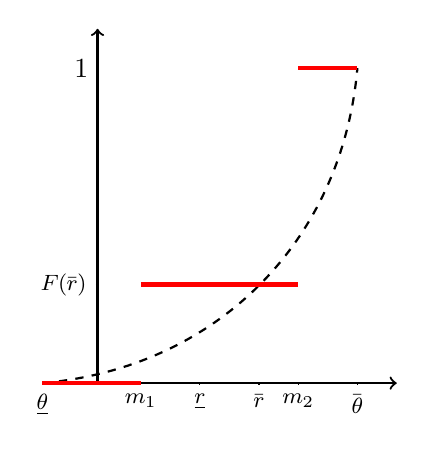
\begin{tikzpicture}[scale=1]
\draw[->, thick] (0,0) -- (4.5,0);
\draw[->, thick] (0.7,0) -- (0.7,4.5) ;
% axis label
\draw [] (4,-.02)node[below]{\footnotesize{$\bar\theta$}}--(4,.02);
\draw [] (0,-.02)node[below]{\footnotesize{$\underline\theta$}}--(0,.02);
\draw [] (2,-.02)node[below]{\footnotesize{$\underline r$}}--(2,.02);
\draw [] (2.75,-.02)node[below]{\footnotesize{$\bar r$}}--(2.75,.02);
\draw [] (3.25,-.02)node[below]{\footnotesize{$m_2$}}--(3.25,.02);
\draw [] (1.25,-.02)node[below]{\footnotesize{$m_1$}}--(1.25,.02);
\draw [] (0.68,1.25)node[left]{\footnotesize{$F( \bar r)$}}--(0.72,1.25);

\draw (0.7,4)node[anchor=east]{1};
% F
\draw[thick, dashed]  (0,0) to [bend right=40](4,4);
\draw[ultra thick, red]  (1.25,1.25) to (3.25, 1.25);
\draw[ultra thick, red]  (0,0) to (1.25, 0);
\draw[ultra thick, red]  (3.25,4) to (4, 4);
\end{tikzpicture}	
\caption{$G^*$ induced by optimal pass/fail.}
\label{fig:passfail}
\end{subfigure}\hspace{0.15\textwidth}
\begin{subfigure}{0.3\textwidth}
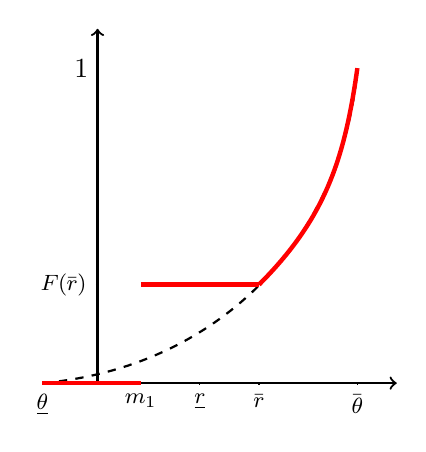
\begin{tikzpicture}[scale=1]
\draw[->, thick] (0,0) -- (4.5,0);
\draw[->, thick] (0.7,0) -- (0.7,4.5) ;
% axis label
\draw [] (4,-.02)node[below]{\footnotesize{$\bar\theta$}}--(4,.02);
\draw [] (0,-.02)node[below]{\footnotesize{$\underline\theta$}}--(0,.02);
\draw [] (2,-.02)node[below]{\footnotesize{$\underline r$}}--(2,.02);
\draw [] (2.75,-.02)node[below]{\footnotesize{$\bar r$}}--(2.75,.02);
\draw [] (1.25,-.02)node[below]{\footnotesize{$m_1$}}--(1.25,.02);
\draw [] (0.68,1.25)node[left]{\footnotesize{$F( \bar r)$}}--(0.72,1.25);

\draw (0.7,4)node[anchor=east]{1};

% F and G
\draw[thick, dashed]  (0,0) to [bend right=40](4,4);
\draw[ultra thick, red]  (1.25,1.25) to (2.75, 1.25);
\draw[ultra thick, red]  (0,0) to (1.25, 0);
% \draw[thick, red]  (2.75, 1.25) to [bend right=19](4,4);
\draw[ultra thick, red]  plot [smooth, tension=2](2.75, 1.25) to [in=262,  out=45](4,4);
\end{tikzpicture}	
\caption{$G^{LC}$ induced by optimal lower-censorship.}
\label{fig:lowercensor}
\end{subfigure}
\caption{The dashed curve corresponds to an arbitrary prior distribution $F$, the red curves correspond to two different posterior-mean distributions that can sustain a stationary equilibrium, and $m_1\triangleq\mathbb{E}_F[\theta|\theta\leq \bar r]$ and $m_2\triangleq\mathbb{E}_F[\theta|\theta> \bar r]$. Note that both distributions are constant on $[\underline r, \bar r]$. }
\label{fig:optdist}
\end{center}
\end{figure}
 
Yet, despite the multitude of equilibrium distributions, all of them have the same distribution on the relevant interval of stopping thresholds $[\underline r,  \bar r]$. Thus, all equilibrium signals induce the same search behavior in the agent. 

\begin{corollary}
\label{cor:1}
If a contract $\langle p, G\rangle\in\mathbb{R}_+\times\mathcal{G}(F)$ can sustain a stationary equilibrium, then $G(m)=F(\bar r)$ for all  $m\in [\underline r, \bar r]$.
\end{corollary}

\autoref{prop:1} characterizes the set of signals that arise in a stationary equilibrium and \autoref{cor:1} shows that all of them are equally valuable to the agent. Additionally, the principal is indifferent across all the equilibrium signals that she can generate, which precludes a unique prediction. Of course, the principal could have preferences over the set of equilibrium signals, for example, if signal production is costly. If the cost of a signal is increasing in the Blackwell order, i.e.,  $\pi$ is more costly than  $\pi'$ if $\pi$ is Blackwell more informative that $\pi'$, then the binary ``pass/fail" signal is the cheapest from the set of signals satisfying \autoref{prop:1}. If the cost of a signal is instead increasing in the number of realizations in its support, then the equilibrium signal is uniquely pinned down by the binary ``pass/fail" signal. This is because any signal with support over just one realization is uninformative, so any contract accepted by the agent in a stationary equilibrium must have support over at least two possible realizations.




\section{Public Signals}\label{public}

Thus far, we have assumed that the agent is  solely dependent on the principal to learn about a good's quality, however, there are settings in which public information is available about the sampled good. In this section,
we consider an agent who learns about a good's quality both by observing 
a signal  $\xi:\Theta\to \Delta (Z)$, where $Z$ is a compact set of signal realizations, and by contracting with the principal. We refer to $\xi$ as a \textit{public signal} because its realizations are observed by both the principal and the agent for free. Without loss of generality, we assume that $\xi$ has full support on $Z$. Additionally, for ease of exposition, we assume that the posterior beliefs conditional on observing any $z\in Z$ are atomless.\footnote{None of our results hinge on this assumption but it does make our proofs less cumbersome.}

We amend the timing of events within any period $t\geq 1$ as follows: First, the agent samples a good of quality $\theta_t$ which is unobserved by  the agent and the principal. However, both observe a public signal realization $z_t\in Z$, which is distributed according to $\xi(\theta_t)$. The principal then offers a  contract $\langle p_t, \pi_t\rangle$ which the agent either accepts or rejects. If the agent accepts the contract $(a_t=1)$, he pays $p_t$ and observes an additional signal realization $s_t\in S$ distributed according to $\pi_t(\theta_t)$. If the agent instead rejects the contract $(a_t=0)$, he pays nothing and observes no additional signal. Finally, the agent decides whether to consume the sampled good and stop searching $(d_t=1)$ or to continue searching $(d_t=0)$. \autoref{fig:timing2} depicts the amended timing of events. 

\begin{figure}[ht]
\centering 
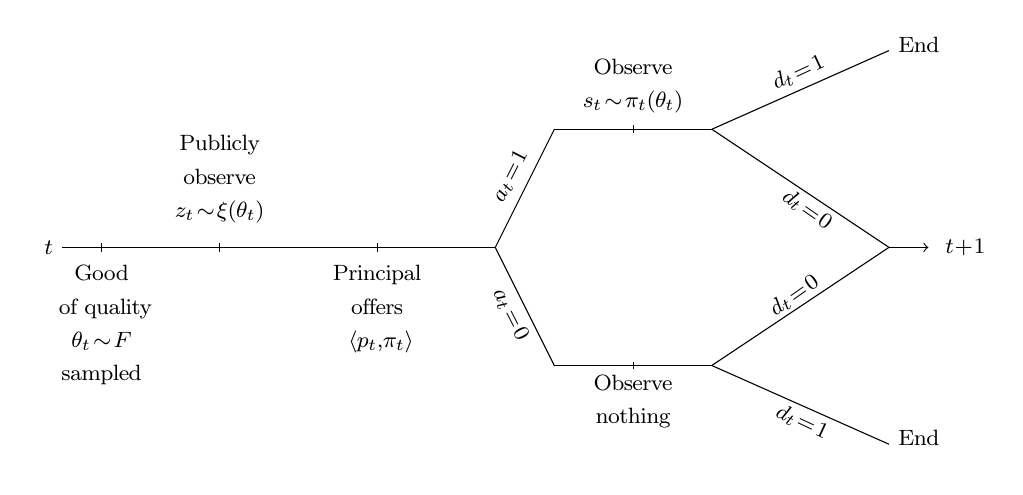
\begin{tikzpicture}[scale=0.5]
\tikzset{
    position label/.style={
             text depth = 1ex
    }
}
    \foreach \x in {-8, -5, -1}
      \draw (\x cm,3pt) -- (\x cm,-3pt);
\draw[-] (-9,0) node[left]{\footnotesize{ $t$}}--(2,0);
\draw[-] (2,0)--(3.5,3);
\draw[-] (2,0)--(3.5,-3);
\draw[-] (3.5,-3)--(7.5,-3);
\draw[-] (3.5,3)--(7.5,3);
\draw[-] (7.5,-3)--(12,0);
\draw[-] (7.5,-3)--(12,-5);
\draw[-] (7.5,3)--(12,5);
\draw[-] (7.5,3)--(12,0);
\draw[->] (12,0)--(13,0)node[right]{\footnotesize{ ${t+1}$}};

\node [position label, align=center, below=3pt] (fend) at (-8,0) {\footnotesize{Good} \\ \footnotesize{ of quality}\\ \footnotesize{$\theta_t\sim F$}\\ \footnotesize{sampled}};
\node [position label, align=center, above=3pt] (fend) at (-5,0) {\footnotesize{Publicly} \\  \footnotesize{observe}\\ \footnotesize{$z_t\sim \xi(\theta_t)$}};
\node [position label, align=center, below=3pt] (fend) at (-1,0) {\footnotesize{Principal} \\ \footnotesize{offers}\\ \footnotesize{ $\langle p_t, \pi_t\rangle$}};
\node [position label, rotate=63, align=center, above] (fend) at (3,1.5) {\footnotesize{$a_t=1$}};
\node [position label, rotate=297, align=center, below] (fend) at (2.8,-1.5) {\footnotesize{$a_t=0$}};


\draw[](5.5,3.1)--(5.5,2.9);
\draw[](5.5,-3.1)--(5.5,-2.9);


\node [position label, align=center, above] (fend) at (5.5,3) {\footnotesize{Observe}\\ \footnotesize{$s_t\sim\pi_t(\theta_t)$}};
\node [position label, align=center, below] (fend) at (5.5,-3) {\footnotesize{Observe}\\ \footnotesize{nothing}};

% \draw[](13,3.1)--(13,2.9);
% \draw[](13,-3.1)--(13,-2.9);
\node [position label, align=center, right] (fend) at (12,5) {\footnotesize{End}};
\node [position label, align=center, right] (fend) at (12,-5) {\footnotesize{End}};

\node [position label, rotate=335, align=center, below] (fend) at (10,-4) {\footnotesize{$d_t=1$}};
\node [position label, rotate=35, align=center, above] (fend) at (10,-1.8) {\footnotesize{$d_t=0$}};

\node [position label, rotate=25, align=center, above] (fend) at (10,3.8) {\footnotesize{$d_t=1$}};
\node [position label, rotate=325, align=center, below] (fend) at (10.2,1.35) {\footnotesize{$d_t=0$}};
  \end{tikzpicture}
  \caption{Timing of events with a public signal}
  \label{fig:timing2}
\end{figure} 

Consider first the case of autarky in which the agent can only observe a realization of the public signal $\xi$. His induced posterior-mean distribution is $G^\xi\in\mathcal{G}(F)$ and his expected payoff in the search market is $u(G^\xi)$, which is the solution to \eqref{eq:1'} when $G=G^\xi$. Note that $u(G^\xi)\geq \underline u$, i.e., the agent's autarky payoff improves in the current setting since he has access to a free signal.

Next, consider the case in which agent can observe the public signal followed by a second signal. Given a public signal realization $z\in Z$, the agent updates his belief from his prior $F$ to an interim belief $F_{z}^{\xi}$. When the agent further updates his belief based on the second signal, $F^\xi_z$ serves as his new ``prior."  Thus, the set of posterior-mean distributions that can be induced through a second signal is the set of mean-preserving contractions of $F^\xi_z$, i.e., $\mathcal{G}(F^\xi_z)$. For example, a fully informative second signal induces $F^{\xi}_z$ itself, whereas an uninformative  second signal induces the degenerate distribution
\[
G^\varnothing_z(m)=\left\{\begin{array}{ccl}
     0 &\mbox{if} & m<\mathbb{E}_{F^\xi_z}[\theta]  \\
     1 &\mbox{if} & m\geq \mathbb{E}_{F^\xi_z}[\theta]  
     \end{array}\right..
\]

% Furthermore, the set of posterior-mean distributions that the principal can induce ex-ante is given by
% \[
% \mathscr{G}\triangleq\left\{\{G_z\}_{z\in Z}: G_z\in \mathcal{G}(F^\xi_z) \text{ for each } z\in Z\right\}.
% \]
 % To distinguish a distribution $G\in \mathcal{G}(F^\xi_z)$ from a family of distibutions  $\{G_z\}_{z\in Z}\mathscr{G}(F,\xi)$, we refer to the former as an \textit{interim}  posterior-mean distribution and to the latter as a \textit{ex-ante-inducible} posterior-mean distributions.   


% Note that for a given family of distributions $\{G_z\}_{z\in Z}$ with $G_z\in \mathcal{G}(F^\xi_z)$ for each $z\in Z$,  the expected posterior-mean distribution $\mathbb{E}_\xi[G_z]$ is a mean-preserving contraction of $F$, i.e., $\mathbb{E}_\xi[G_z]\in\mathcal{G}(F)$, and $G^\xi$ is a mean-preserving contraction of $\mathbb{E}_\xi[G_z]$.\footnote{$\mathbb{E}_{\xi}[G_z]=\int_Z G_z \xi(dz)=\int_\Theta\int_Z G_z \xi(dz|\theta)dF(\theta)$. The two conditions follow from Theorem 3.A.12(b) \cite{sha07}.} The converse however is not true, i.e., given a distribution $G\in \mathcal{G}(F)$ such that $G^\xi$ is a mean-preserving contraction of $G$, it is possible that there is no family of distributions $\{G_z\}_{z\in Z}$ with $G_z\in \mathcal{G}(F^\xi_z)$ for each $z\in Z$ 


% The reader may therefore think that the contracting problem with a public signal $\xi$ is isomorphic to the contracting problem of the baseline model but with an additional constraint that the principal  choose a distribution $G\in\mathcal{G}(F)$ such that $G^\xi$ is a mean-preserving contraction of $G$.

% Unfortunately, 
% The converse however is not true, i.e., not every $G\in \mathcal{G}(F)$ such that $G^\xi$ is a mean-preserving contraction of $G$ can be represented as the expected posterior-mean distribution 




% Thus, the contracting problem with a public signal cannot be reduced to simply choosing a distribution $\widehat G\in\mathcal{G}(F)$ such that $G^\xi$ is a mean-preserving contraction of $\widehat G$. 


% \begin{lemma}
% \label{lemma:3}
% Given a family of distributions $\{G_z\}_{z\in Z}\in \mathscr{G}$, the expected posterior-mean distribution $\mathbb{E}_\xi[G_z]$ is an element of  $\mathcal{G}(F)$ and is Blackwell more informative than $G^\xi$. Conversely, given a distribution $G\in \mathcal{G}(F)$ that is Blackwell more informative than $G^\xi$, there exists a family of distributions $\{G_z\}_{z\in Z}\in \mathscr{G}$ such that $G=\mathbb{E}_{\xi}[G_z]$.
% \end{lemma}

Therefore, following a public signal realization $z\in Z$, the principal can propose any contract of the form $\langle p, G\rangle\in\mathbb{R}_+\times \mathcal{G}(F^\xi_z)$. Our goal is to characterize stationary equilibrium outcomes. However, we must first update the conditions  for a stationary equilibrium given in \autoref{def:1} to account for the agent's ability to learn from the public signal.  

\begin{definition}
    \label{def:2}
    \normalfont Given a public signal $\xi$, a stationary equilibrium  is defined by a pair of agent-principal continuation values $(U, V)\in \mathbb{R}^2$ and a family of  contracts $\{\langle p_z,G_z\rangle\}_{z\in Z}$ with $\langle p_z, G_z\rangle\in\mathbb{R}_+\times \mathcal{G}(F^\xi_z)$ for each $z\in Z$ such that in each period and after every history:
    \begin{enumerate}
    \item The agent stops searching and consumes a good of expected quality $m\in \Theta$ if and only if $m>\delta U$, i.e.,  \eqref{eq:os} holds,  

    \item Given a public signal realization $z$, the agent accepts  $\langle \widehat p,\widehat G\rangle\in\mathbb{R}_+\times\mathcal{G}(F^\xi_z)$  if and only if
    \begin{align*}
          \label{eq:pc2}
    \tag{PC$^\xi_z$}
           c_{\widehat G}(\delta U)-c_{G_z^\varnothing}(\delta U) \geq \widehat p,
    \end{align*}
       
\item Given a public signal realization $z$, the principal proposes $\langle p_z,G_z\rangle$ to maximize her profit, i.e.,
\[
\label{eq:pm2}
\tag{PM$^\xi_z$}
 \langle p_z,G_z\rangle\in \argmax_{\langle \widehat p, \widehat G\rangle\in\mathbb{R}_+\times \mathcal{G}(F^\xi_z)}\hspace*{.2em} \widehat p+ \widehat G(\delta U) \delta V \hspace*{.5em} \text{ subject to \eqref{eq:pc2}},
\]   
\item Payoffs are self-generating, i.e.,
\[
\label{eq:sga2}
\tag{SG-A$^\xi$}
U=\mathbb{E}_\xi[\delta U+c_{G_z}(\delta U)-p_z] 
\] 
    and
    \[
    \label{eq:sgp2}
\tag{SG-P$^\xi$}
V= \mathbb{E}_\xi[p_z + G_z(\delta U) \delta V].
\] 
\end{enumerate}
\end{definition} 

In a stationary equilibrium, the agent and the principal anticipate the continuation values $U$ and $V$ in each period following any history of events. Since the anticipated continuation values are independent of the observed public signal realizations, the agent's optimal stopping rule is still given by \eqref{eq:os}. Upon observing the public signal realization $z\in Z$, the agent updates his belief to $F^\xi_z$ and accepts any contract that gives him a higher payoff than
 $\delta U+c_{G^\varnothing_z}(\delta U)=\max\{\mathbb{E}_{F^\xi_z}[\theta], \delta U\}$, which is the payoff he gets by either consuming the good in the current period without observing a second signal or by waiting for the next period. The constraint \eqref{eq:pc2} captures the agent's contract acceptance decision.
 
 Given the anticipated continuation values and the agent's strategies, the principal  proposes a contract $\langle p_z, G_z\rangle\in\mathbb{R}_+\times \mathcal{G}(F^\xi_z)$ after each public signal realization $z\in Z$ in order to maximize her profit, as given in \eqref{eq:pm2}. Finally, the anticipated continuation values must be consistent with the agent's and principal's stationary equilibrium strategies, which is captured by \eqref{eq:sga2} and \eqref{eq:sgp2}. 

In order to state our main result of this section, we must first introduce some notation. Given a public signal realization $z\in Z$, we denote the lower and upper bounds on the support of $F^\xi_z$ by $\underline \theta_z\triangleq\inf \hspace*{.2em} \supp(F^\xi_z)$ and $\bar \theta_z\triangleq\sup \hspace*{.3em}\supp(F^\xi_z)$ respectively, and let
\[
Z_A\triangleq\{z\in Z:r^\xi \hspace*{.1em} < \hspace*{.1em}\underline \theta_z\}.
\]
In the case that $r^\xi\in [\underline\theta_z, \bar\theta_z]$, let 
$\bar x_z\triangleq\sup\{x\in [\underline\theta_z, \bar\theta_z]:\mathbb{E}_{F_z^\xi}[\theta|\theta\leq x]\leq r^\xi\}$, and for some $k\geq 0$, let 
\[
Z_B(k)\triangleq\{z\in Z:r^\xi\in [\underline \theta_z ,\bar\theta_z]\hspace*{.1em} \wedge \hspace*{.1em}\bar x_z\hspace*{.1em} < \hspace*{.1em}\bar r-k\}.
\]
Note that $Z_A$ and $Z_B(k)$ could be empty. Finally, we define  the function $\Phi:\mathbb{R}_+\to \mathbb{R}$ by
\small{\begin{align*}
        \label{eq:5}
        \tag{5}
&\Phi(k)\\
\triangleq &-\int_{\bar r-k}^{\bar r}\big(1-F(m)\big)dm+\int_{Z_A}\int_{r^\xi}^{\bar r-k}F^\xi_z(m)dm \xi(dz)+\int_{Z_B(k)}\int_{\bar x_z}^{\bar r -k}\big(F^\xi_z(m)-F^\xi_z(\bar x_z)\big)dm\xi(dz).
        \end{align*}} %%
       \normalsize 
We provide a detailed discussion of  $Z_A$, $Z_B(\cdot)$, and $\Phi(\cdot)$ following the statement of the following theorem.

\begin{theorem}
\label{prop:2}
    For any public signal $\xi:\Theta\to \Delta(Z)$, a stationary equilibrium exists. Furthermore, in any stationary equilibrium, 
    \begin{enumerate}[$(i)$]
        \item $U=u(G^\xi)$ and
        \item $V=\bar u-u(G^\xi)-\displaystyle\frac{k^*}{\delta}$, where $k^*\in [0, \bar r-r^\xi]$ is the unique solution to the fixed point 
        \[
        k=\frac{\delta}{1-\delta}\Phi(k).
        \]
    \end{enumerate}
\end{theorem}

\autoref{prop:2} establishes that for any given public signal, a stationary equilibrium exists and that all stationary equilibria are payoff equivalent. The agent gets his autarky payoff $u(G^\xi)$, which is now (potentially strictly) higher than $\underline u$, whereas the principal's payoff may be (potentially strictly) lower than the maximal surplus that she could feasibly extract $\bar u-u(G^\xi)$.


The proof of \autoref{prop:2} demonstrates that in equilibrium, the principal can restrict her attention to pass/fail signals with a cutoff structure such that a good ``passes" if and only if its  quality falls above a cutoff, which potentially depends on the realization of the public signal, and the agent is persuaded to stop his search if and only if he observes a ``pass." In other words, the induced stopping threshold is the same as the cutoff. This mirrors the finding in \autoref{prop:1}, wherein the principal could offer pass/fail signals with a cutoff of $\bar r$. However, in contrast to \autoref{prop:1}, the principal may no longer be able to induce the efficient stopping threshold $\bar r$ following every public signal realization, in which case she fails to generate and extract the full surplus. The loss of surplus stemming from the difference between the stopping thresholds induced in a stationary equilibrium and $\bar r$  is characterized by $k^*$.

To see why, suppose the principal seeks to induce a  stopping threshold $\bar r - k$ for some $k\geq 0$ in a stationary equilibrium. The change in total surplus that can be extracted by the principal from inducing $\bar r-k$ instead $\bar r $ is captured by the first term in \eqref{eq:5}. However, given the agent's actual reservation value in a stationary equilibrium is $\delta u(G^\xi)=r^\xi$, the principal may not be able to induce the  desired stopping threshold $\bar r-k$. In particular, there are two cases when the principal fails to induce $\bar r-k$ after some realization $z\in Z$ of the public signal. First, if $r^\xi<\underline \theta_z$, then the lowest quality the agent expects to receive when he observes $z$ is above his autarky reservation value. Hence, the agent is too optimistic and he  terminates his search regardless of the contract offered by the principal. This occurs when $z\in Z_A$ and the efficiency loss in this case is captured by 
 \[
 \int_{Z_A}\int_{r^\xi}^{\bar r-k}\big(F^\xi_z(m)-F^\xi_z(r^\xi)\big)dm,
 \]
 which yields the second term in \eqref{eq:5} after noting that $F^\xi_z(r^\xi)=0$ for all $z\in Z_A$. Second, if $r^\xi\in [\underline \theta_z ,\bar\theta_z]$, the principal can only induce stopping thresholds below $\bar x_z$.\footnote{For example, a pass/fail signal with a cutoff above $\bar x_z$ would not persuade the agent to continue searching if he observes a ``fail."} Hence, if $\bar x_z < \bar r-k$, the best the principal can do is induce a stopping threshold of $\bar x_z$ instead of $\bar r-k$. This occurs when $z\in Z_B(k)$ and the efficiency loss is captured by the last term in \eqref{eq:5}.
    
Therefore, following public signal realizations in $Z_A\cup Z_B(k),$ the principal must make concessions, which lower her continuation payoff. The proof of \autoref{prop:2} shows that the loss in the principal's equilibrium payoff from these concessions are quantified by  the unique solution to the fixed point $k=\frac{\delta}{1-\delta}\Phi(k)$.


%\tm{ Then maybe finish with an example of how this works for uniform distribution. }
Note that when $Z_A=Z_B(0)=\emptyset$, then $\Phi(0)=0$ by construction, which implies that the principal induces the efficient stopping threshold following every $z\in Z$ and, by \autoref{prop:2}, extracts the full surplus. For example, when $F_z^\xi$ has full support over $\Theta$ for all realizations $z\in Z,$ the set $Z_A$ is trivially empty. The following result provides a sufficient and necessary condition for $Z_B(0)$ to also be empty in this case. 
    
 
   
\begin{corollary}\label{cor:2}
        Consider a public signal $\xi:\Theta\to \Delta(Z)$ such that $F_z^\xi$ has full support on $\Theta$ for almost all $z\in Z$. The principal extracts the socially efficient surplus in a stationary equilibrium if and only if $\mathbb{E}_{F_z^\xi}[\theta|\theta\leq \bar r]\leq r^\xi$ for almost all $z\in Z$.
\end{corollary}

Intuitively, the requirement that $\mathbb{E}_{F_z^\xi}[\theta|\theta\leq \bar r]\leq r^\xi$ for almost all $z\in Z$ imposes ``fat" left tails of the interim beliefs following almost every public signal realization. This condition is trivially satisfied when $\xi$ is uninformative as $\mathbb{E}_F[\theta|\theta\leq \bar r]\leq \underline r\leq r(G)$ for any $G\in\mathcal{G}(F)$ and any absolutely continuous prior $F$. Hence, our result in \autoref{prop:1} can be seen as a special case of \autoref{prop:2}.

% \section*{\bph{Discussion: Points to add, perhaps here, perhaps sprinkled throughout}}

% Our analysis has centered around situations in which the planner has access to more information than the agent. We briefly highlight two market features that can undermine this assumption, and suggest directions for future research.

% First, in some markets it may be costly for the principal to prepare more informative signal structures, representing that the principal may not have easy access to all information about object quality. It is not obvious how to model such situations. One approach is to model a cost as increasing in the number of signal realizations in the support of the contracted structure. As any signal structure with support over just one report is uninformative, any contract accepted by the agent in a stationary equilibrium must have support over at least two possible realizations; therefore, our main result goes through and the signal structure is uniquely pinned down by a binary ``pass/fail" test, which is the cheapest test allowable in equilibrium. \tm{say something about the lower censorship test} Another approach is to create a partial order over the costs of signal structures in which a signal structure $\pi$ is more costly than signal structure $\pi'$ if $\pi$ is Blackwell more informative that $\pi'$. In this setting, a binary ``pass/fail" test is the cheapest test that achieves the socially efficient outcome in equilibrium. Of course, there are many other ways to conceive of costs, and the analysis of costs in an information design framework (with or without search) is an important area for future research.

% Of course, in some markets the agent may also observe a private signal about the quality of each object before deciding to contract with the principal. \bph{Alt that fixes punctuation and changes the unwieldy ``signal structure" language. I'm not sure about the word ``potentially" which I added since I don't think screening is necessarily the outcome (i.e. it's not obvious if we HAVE to allow the principal to offer a menu): The agent's willingness to pay for additional information would then be his private information, potentially(?) inducing a screening problem \citep[as in][]{mus78} into each stage game between the principal and the agent.} \tm{As I see it, it is a screening problem if we don't want to restrict the space of mechanisms. It could of course be that the principal chooses not to screen. But that is a result. For example, in the Myerson monopoly pricing problem, the principal's profit maximization is set up as a screening problem even though the optimal mechanism is a simple posted-price.}\bph{got it, let's go with your suggestion}The agent's willingness-to-pay for additional signal structures \tm{``...additional signal"? Saying ``additional \textbf{information} would then be his private \textbf{information}..."\bph{got it, happy to go with your wording. Do you think it should be ``additional signal" or ``an additional signal"?} may be confusing} would then be his private information, introducing a screening problem \citep[as in][]{mus78} into each stage game between the principal and the agent. Such an analysis would require a different set of tools; for example, truth-telling constraints for a privately-informed agent would be more tractable if formulated via recommendation mechanisms \citep[as in][]{kol17} rather than via distributions of posterior means as in our analysis. We therefore view the study of private signals in search markets with endogenously-supplied information as a fruitful avenue for future research.

Of course, in some markets the agent may also observe a private signal about the quality of each object before deciding to contract with the principal. The agent's willingness-to-pay for an additional signal would then be his private information, introducing a screening problem \citep[as in][]{mus78} into each stage game between the principal and the agent. Such an analysis would require a different set of tools; for example, truth-telling constraints for a privately-informed agent would be more tractable if formulated via recommendation mechanisms \citep[as in][]{kol17} rather than via distributions of posterior means as in our analysis. We therefore view the study of private signals in search markets with endogenously-supplied information as a fruitful avenue for future research.


% Such analysis would also require a different set of tools; for example, truth-telling constraints for a privately informed agent would be more tractable if formulated via recommendation mechanisms \citep[as in][]{kol17} rather than via distributions of posterior means as in our analysis. \bph{Possibly include something formal in appendix, following the discussion/example about how posterior means don't capture informativeness necessarily. If so, we can add a sentence here saying something like ``we expand upon these technical considerations in the appendix."} We also view the study of private information in search markets with endogenously-supplied information as a fruitful avenue for future research.

\section{Conclusion}\label{conclude}


We consider a simple \emph{persuaded search} game between an uninformed searching agent and a profit-maximizing principal who can sell an informative signal but lacks commitment power across periods. Our model highlights novel inter- and intra-temporal trade-offs that arise due to the dynamic considerations for both the principal and agent. We show that in the essentially unique stationary equilibrium, the principal fully extracts the socially efficient surplus in the search market by selling a signal that pools low quality objects into a ``fail" category, and extracts the surplus through dribs and drabs. 

Limiting attention to stationary strategies and removing commitment power restrict the principal. % and lower her equilibrium payoffs. 
The former precludes more complicated contracts that condition the current proposal on the history of past contracts, agent's decisions, and signal realizations. Similarly, a principal with long-term commitment power can sustain a larger set of contracts in equilibrium. For example, the principal could ``sell" the signaling technology to the agent in the first period at price equal to the full surplus.\footnote{Formally, the principal could propose a sequence of contracts $\langle p_t, G_t\rangle_{t\geq 1}$ such that $G_t=F$ for all $t\geq 1$, $p_t=0$ for all $t>1$, and $p_1=\bar u-\underline u$. Such a sequence of contracts cannot be implemented without commitment as  the principal would deviate away from charging $p_t=0$  in periods $t>1$, and thus, the agent would never accept the contract.} Yet, our \autoref{prop:1} finds that the principal has no value for either non-stationary contracts or commitment power as she is able to sustain the highest possible equilibrium payoffs via a simple spot contract that is constant across time. Possibly relatedly, information brokers in some real-world search markets offer stationary contracts with no commitment to contracts in the future.\footnote{For example, searchers for used cars can purchase a Carfax report for a car (which is not tailored to an individual's search history) with no agreement on future reports.}  %\zma{I think the point about commitment is a very interesting insight of the analysis. We should discuss it after Theorem 1, especially because the public-signal case will be between Theorem 1 and the conclusion.}\bph{I think we should keep the discussion here, to keep the body streamlined. We make this point in the intro, and now we're bookending the paper with it. It's also nice that there isn't much between Theorem 1 and conclusion (even with the addition of public signals), so I don't think the reader will be confused.}

%In ongoing work we study the set of all equilibria, which potentially involve non-stationary strategies. Using techniques from the repeated game literature, we show that the set of equilibria expand as the discount rate rises. Optimal signals continue to follow a ``pass-fail" structure in which the agent stops only when an object ``passes" the test. Below a certain discount factor threshold, the stationary equilibrium we characterize in the current paper is the unique equilibrium. As the discount rate rises beyond this threshold, the set of equilibrium payoffs expands, and admits less efficient equilibria. In the limit or arbitrarily high patience, a folk-theorem-like result emerges: nearly any payoffs satisfying individual rationality can be sustained in equilibrium.

In ongoing work, we study the set of all equilibrium payoffs as a function of the discount factor. We show that for sufficiently low values of $\delta$, all equilibria are payoff equivalent to the stationary equilibrium we characterize in \autoref{prop:1}, whereas for sufficiently high values of $\delta$, equilibrium payoffs emerge that can only be supported by non-stationary strategies. However, optimal signals continue to follow a ``pass/fail" structure.

Our analysis builds on a workhorse model of sequential random search in which the agent is searching over non-strategic objects. Of course, some search markets will contain different salient features that are not present in our model. For example, some matchmakers in the heterosexual dating market solicit payments only from searchers of a particular sex, while others charge both sexes.\footnote{\cite{matchmaker}, \textit{Why Women Must Pay For Matchmaking}, \hyperlink{https://medium.com/@stevenbward/why-women-must-pay-for-matchmaking-a8648372d055}{https://medium.com/@stevenbward/why-women-must-pay-for-matchmaking-a8648372d055}.} The features of equilibrium contracts may therefore differ, and further study may yield novel economic insights. 


% \zma{One aspect that is left out of our model that could be interesting is learning (probably a different paper). This is possibly one of the reasons why commitment and no commitment yield the same payoffs; there is nothing to learn from one period to the next one. In some applications, the principal could learn valuable information and use it in future contracts. One (very basic) example is in the spirit of Kolotilin et al 2017 (ECMA), which studies a receiver with payoff-relevant private information and a sender designing a mechanism that conditions the information structure on the receiver's report of her private information.}

% \zma{In our setup, it could be that the agent has a sampling cost that is unknown to the sender. The sender could ask, at the beginning, what is the receiver's cost, then tailor an information structure. This makes sense because if the sampling cost is high, for instance, it will be harder to stream along the search, so maybe it is a good idea to provide more information as soon as possible, charge a lot for it, and be done. However, the agent knows this, so it will have incentive to over-report her cost. As the search evolves, however, the principal may want to experiment a little bit to confirm the agent's cost. Maybe she does not offer a lot of information today, and if the agent rejects the object and samples again, now the principal learned that the true sampling cost must be smaller than reported. Then, it makes sense to adjust the contract. Commitment would not allow for this, hence, in this world the principal could do better without commitment.}

% \zma{A different source of uncertainty comes from the value of hiring. If we think about a consulting company (principal) analyzing different investment projects proposed by a client (agent), depending how the profits of the company are evolving (an exogenous state variable only the agent observes), it may value more or less a given quality level (e.g., if the company is doing well, I can take more risks; if the company is doing bad, I can only afford to take a banger). In this world, the principal could ask the agent every period to report the state of the world, before offering a contract. As in Kolotilin 2017, the agent may strategically misreport trying to influence the information structure she receives.}


% We conclude this section by commenting on stationarity and our assumption of limited commitment. Plainly, restricting attention to stationary strategies is limiting as the intermediary could have opted for a non-stationary strategy that conditions the current contract proposal on past contracts, on the firm's past choices, and on the scores of previous workers. Yet, we know from \autoref{prop:1} that restricting attention to stationary strategies is without loss of optimality, as the intermediary is able to sustain the highest possible equilibrium payoffs through stationary strategies alone. 


% Similarly, an intermediary with long-term commitment power can sustain a larger set of contracts in equilibrium. For example, the intermediary could propose a sequence of contracts $\langle p_t, G_t\rangle_{t\geq 0}$ such that $G_t=F$ for all $t\geq 0$, $p_t=0$ for all $t\geq 1$, and $p_0=\bar u-\underline u$, which is akin to an intermediary that ``sells" its signaling technology to the firm in period $t=0$, thereby extracting the maximal value of information at once. Such a sequence of contracts cannot be implemented without commitment; the intermediary would want to deviate away from charging $p_t=0$  in periods $t\geq 1$, and thus, the firm would never accept the contract in the initial period. Yet, by \autoref{prop:1}, the intermediary has no value for  commitment as it is able to sustain the highest possible equilibrium payoffs via spot contracts alone.

  
\singlespacing
 \bibliographystyle{abbrvnat}
\nocite{}\bibliography{bibref}
\onehalfspacing

\section*{Appendix}\label{appendix}

\noindent\begin{proof}[Proof of \autoref{lemma:1}]
If the agent never searches, i.e., $\underline u=\bar u$, then $\bar u=m_\varnothing$ because $\underline u=\max\{m_\varnothing, 0\}$ and $\bar u>0$. Suppose for contradiction that $\underline \theta<\delta m_\varnothing$. Because $\bar u =m_\varnothing$ and because $\bar u$ is the solution to \eqref{eq:1} with $G=F$, we must have 
\begin{align*}
m_\varnothing=\int_\Theta \max\{m,\delta m_\varnothing\}dF(m)>\int_\Theta m dF(m) =m_\varnothing,
\end{align*}
where the strict inequality follows from $F$ having positive mass over the range $[\underline \theta, \delta m_\varnothing]$, and the second equality follows from the definition of $m_\varnothing$. This however yields the contradiction $m_\varnothing>m_\varnothing$. Hence, if the agent never searches then $\underline \theta\geq \delta m_\varnothing$.


Conversely, suppose $\underline\theta\geq \delta m_\varnothing$. Then for any $G\in\mathcal{G}(F)$, 
\begin{align*}
\int_\Theta\max\{m, \delta m_\varnothing\} dG(m)=\int_\Theta mdG(m)=m_\varnothing.
\end{align*}
Hence, $m_\varnothing$ is the solution to the fixed point problem in \eqref{eq:1}, i.e., $u(G)=m_\varnothing$ for all $G\in\mathcal{G}(F)$. In particular, $\bar u\triangleq u(F)=u(G^\varnothing)\triangleq\underline u$, so the agent never searches. 
\end{proof}\\

\noindent \begin{proof}[Proof of \autoref{lemma:2}]
\begin{enumerate}[$(i)$]
    \item $G^*$ is a mean-preserving contraction of $F$, so $c_{G^*}\leq c_F$ pointwise with
    \begin{align*}
        c_{G^*}(\bar r)&=\int_{\bar r}^{\bar\theta}(m-\bar r)dG^*(m)\\[6pt]
        &=\big(\mathbb{E}_F[\theta|\theta>  \bar r]-\bar r\big)(1-F(\bar r))\\[6pt]
        &=\int_{\bar r}^{\bar\theta}(m-\bar r)dF(m)\\[6pt]
        &=c_F(\bar r),
    \end{align*}
    where the first and last equality follow from integration by parts, and the second equality follows by rewriting the first integral using the definition of $G^*$ in \eqref{eq:3}. Additionally, 
    \[
    \partial_+c_{G^*}(\bar r)=G^*(\bar r)-1=F(\bar r)-1=\partial_+c_F(\bar r),
    \]
    where the first and last equality follow by definition of the right-derivative of $c_G$ for $G=G^*$ and $G=F$ respectively, and the second equality follows by the definition of $G^*$ in \eqref{eq:3}. Hence, $c_{G^*}(x)\leq c_F(x)$ for all $x\in \Theta$ with a point of tangency at $x=\bar r$.

    \item 
    $r(G^*)$ is the unique solution to \eqref{eq:2} with $G=G^*$, and $r(F)$ is the unique solution to \eqref{eq:2} with $G=F$. In particular, 
    \[
    r(F)=\left(\frac{\delta}{1-\delta}\right)\cdot c_F\big(r(F)\big)=\left(\frac{\delta}{1-\delta}\right)\cdot c_{G^*}\big(r(F)\big),
    \]
where the first equality follows from \eqref{eq:2}, and the second inequality follows from point $(i)$ of \autoref{lemma:2} and the fact that $r(F)=\bar r$ by definition. This implies that $r(F)$ must also be a solution to the fixed point problem in \eqref{eq:2} with $G=G^*$, i.e., $r(G^*)=r(F)=\bar r$.

\item From part $(ii)$ of \autoref{lemma:2}, $r(G^*)=\bar r$, which implies that $r(G^*)\geq r(G)$ for all $G\in\mathcal{G}(F)$. 
% We will show that for any binary distribution $ G$ with $r(G)=r(G^*)$, it is necessarily the case that $G=G^*$, thereby proving that $G^*$ is the unique binary distribution that induces the efficient reservation value. 
Consider a binary distribution $\widehat G\in\mathcal{G}(F)$ with $r(\widehat G)=\bar r$. Let the support of $\widehat G$ be $\{m_1, m_2\}$ with $m_1<m_\varnothing<m_2$. Our goal is to show that $\widehat G=G^*$.

To that end, we first express $c_{\widehat G}$ as
\[
c_{\widehat G}(x)=\left\{\begin{array}{ccl}
     m_\varnothing-x& \mbox{if} &~~~ x\leq m_1 \\
    (m_2-x)(1-\widehat G(m_1))& \mbox{if} &~~~ x\in[ m_1, m_2] \\
     0& \mbox{if} &~~~ x\geq m_2 \\
\end{array} \right..
\]
Notice that $c_{\widehat G}(x)=c_{G^\varnothing}(x)$ for all $x\in [\underline\theta, m_1]\cup [m_2, \bar \theta]$ by construction. 

We want to show that $\bar r\in (m_1, m_2)$. Suppose to the contrary that $\bar r\in[\underline\theta, m_1]\cup [m_2, \bar \theta]$. We then would have 
\[
\bar r=\left(\frac{\delta}{1-\delta}\right)\cdot c_{\widehat G}(\bar r)=\left(\frac{\delta}{1-\delta}\right)\cdot c_{G^\varnothing}(\bar r),
\]
where the first equality follows by the fact that $\bar r=r(\widehat G)$, and the second follows because $\bar r\in [\underline\theta, m_1]\cup [m_2, \bar \theta]$ by assumption. However, the above equality implies that $\bar r=r(G^\varnothing)=\underline r$, which is a contradiction of $\bar r>\underline r$ by \hyperref[ass:1]{Assumption 1}. Hence, $\bar r\in (m_1, m_2)$. 

Because $\widehat G$ is a mean-preserving spread of $F$ and because $\bar r$ is the unique solution to the fixed-point problem in  \eqref{eq:2} for both $G=F$ and $G=\widehat G$, we have that $c_{\widehat G}(x)\leq c_F(x)$ for all $x\in\Theta$ with a point of tangency at $x=\bar r$. Additionally, because both $c_F$ and $c_{\widehat G}$ are differentiable in an open neighborhood of $\bar r$, the former by the absolute continuity of $F$ and the latter by its linearity over $(m_1, m_2)$, we can exploit the tangency of $c_F$ and $c_{\widehat G}$ at $\bar r$ to conclude that 
\[
\underbrace{\partial_+c_F(\bar r)}_{F(\bar r)-1}=\underbrace{\partial_+c_{\widehat G}(\bar r)}_{\widehat G(m_1)-1}.
\]
In other words, $F(\bar r)=\widehat G(m_1)$. Then
\begin{align*}
    c_F(\bar r)&=c_{\widehat G}(\bar r)\\[6pt]
    \Leftrightarrow \int_{\bar r}^{\bar \theta} (m-\bar r)dF(m)& = (m_2-\bar r)(1-\widehat G(m_1))\\[6pt]
    \Leftrightarrow \big(\mathbb{E}_F[\theta|\theta>\bar r]-\bar r\big)(1-F(\bar r))& = (m_2-\bar r)(1-F(\bar r))\\[6pt]
    \Leftrightarrow \mathbb{E}_F[\theta|\theta>\bar r]&= m_2.
\end{align*}
Finally, $\widehat G$ being a mean-preserving contraction of $F$ implies that 
\begin{align*}
    m_\varnothing&=m_1 \widehat G(m_1)+m_2(1-\widehat G(m_1))=m_1 F(\bar r)+\mathbb{E}_F[\theta|\theta>\bar r](1-F(\bar r)),
\end{align*}
which implies that $m_1=\mathbb{E}_F[\theta|\theta\leq \bar r]$.  

We have thus far shown that $\widehat G=G^*$ as given in \eqref{eq:3}. In other words, if a binary distribution $G\in \mathcal{G}(F)$ satisfies $r(G)=\bar r$, then $G=G^*$. Hence, $G^*$ is the unique binary distribution that attains the efficient reservation value.  

\item By construction, $G^*$ has mass only at $\mathbb{E}_F[\theta|\theta\leq \bar r]$ and $\mathbb{E}_F[\theta|\theta>  \bar r]$. Thus, proving that $G^*(m)=F(\bar r)\in (0,1)$ for all $m\in [\underline r, \bar r]$ is equivalent to showing that
\[
\mathbb{E}_F[\theta|\theta\leq \bar r]<\underline r<\bar r<\mathbb{E}_F[\theta|\theta>  \bar r].
\] 
Because $F$ has full support, it is clear that $\mathbb{E}_F[\theta|\theta\leq \bar r]<\bar r<\mathbb{E}_F[\theta|\theta>  \bar r]$. From \hyperref[ass:1]{\Cref{ass:1}}, we also have $\bar r>\underline r$. Hence, to prove the statement in the lemma, we just need to show that $\mathbb{E}_F[\theta|\theta\leq \bar r]<\underline r$. 

Suppose for contradiction that $\mathbb{E}_F[\theta|\theta\leq \bar r]\geq \underline r$. Then
\begin{align*}
\bar r&=\left(\frac{\delta}{1-\delta}\right)\cdot c_{G^*}(\bar r)\\[6pt]
&\leq \left(\frac{\delta}{1-\delta}\right)\cdot c_{G^*}(\mathbb{E}_F[\theta|\theta\leq \bar r])\\[6pt]
&=\left(\frac{\delta}{1-\delta}\right)\cdot c_{G^\varnothing}(\mathbb{E}_F[\theta|\theta\leq \bar r])\\[6pt]
&\leq \left(\frac{\delta}{1-\delta}\right)\cdot c_{G^\varnothing}(\underline r)\\[6pt]
&=\underline r,
\end{align*}
where the first equality follows because $\bar r=r(G^*)$ is the unique solution to \eqref{eq:2} with $G=G^*$, the first inequality follows because $c_{G^*}$ is weakly decreasing and $\bar r>\mathbb{E}_F[\theta|\theta\leq \bar r]$, the second equality follows because $c_{G^*}(x)=c_{G^\varnothing}(x)$ for all  $x\in \big[\underline \theta, \mathbb{E}_F[\theta|\theta\leq \bar r]\big]\cup \big[\mathbb{E}_F[\theta|\theta>\bar r], \bar \theta\big]$, the last inequality follows because $c_{G^\varnothing}$ is weakly decreasing and $\underline r\leq \mathbb{E}_F[\theta|\theta\leq \bar r]$ by assumption, and the last equality follows because $\underline r=r(G^\varnothing)$ is the unique solution to \eqref{eq:2} with $G=G^\varnothing$. However, this yields the contradiction that $\bar r\leq \underline r$. Hence, $\mathbb{E}_F[\theta|\theta\leq \bar r]<\underline r$, which concludes the proof. 
\end{enumerate} \end{proof}\\

\noindent\begin{proof}[Proof of \autoref{cor:1}]
From Point $(iv)$ of \autoref{prop:1}, any  $G\in\mathcal{G}(F)$ that sustains a stationary equilibrium must satisfy $G( \underline r)=F(\bar r)$, which implies that $\partial_+ c_G( \underline r)=F(\bar r)-1$. Additionally, from Point $(v)$ of \autoref{prop:1}, $c_G\geq c_{G^*}$  
pointwise. We also have $c_F\geq c_G$ pointwise for any $G\in\mathcal{G}(F)$. By construction, $c_F(\bar r)=c_{G^*}(\bar r)$, and $\partial_+ c_F( \bar r)=\partial_+ c_{G^*}( \bar r)=F(\bar r)-1$. Since $c_G$ is sandwiched between $c_F$ and $c_{G^*}$, we have $\partial_+ c_G( \bar r)=F(\bar r)-1$ as well. 
Finally, by the convexity of $c_G$ (see point $(c)$ of \autoref{remark:1}), we have 
\[
\underbrace{\partial_+ c_G(\underline r)}_{=F(\bar r)-1}\hspace*{.5em}\leq \hspace*{.5em}\underbrace{\partial_+ c_G(x)}_{=G(x)-1}\hspace*{.5em}\leq \hspace*{.5em}\underbrace{\partial_+ c_G(\bar r)}_{=F(\bar r)-1}
\]for all $x\in [\underline r, \bar r]$. Equivalently, $G(x)=F(\bar r)$ for all $x\in [\underline r,  \bar r]$.
\end{proof}\\

% \noindent\begin{proof}[Proof of \autoref{lemma:3}]
%    Fix a family of distributions $\{G_z\}_{z\in Z}\in \mathscr{G}$. For each $z\in Z$, $G^\varnothing_z$ is a mean-preserving contraction of $G_z$, and $G_z$ is a mean-preserving contraction of $F_z^\xi$.   Since mean-preserving contractions are closed under mixtures (Theorem 3.A.12(b), \cite{sha07}), $G^\xi=\mathbb{E}_\xi[G^\varnothing_z]$ is a mean-preserving contraction of $\mathbb{E}_\xi[G_z]$, and $\mathbb{E}_\xi[G_z]$ is a mean-preserving contraction of $\mathbb{E}_\xi[F^\xi_z]=F$. In other words, $\mathbb{E}_\xi[G_z]\in \mathcal{G}(F)$ and is Blackwell more informative than $G^\xi$, which completes the first statement of the lemma.

% Before we prove the second statement of the lemma, we first introduce some notation. Let $\mathcal{B}(\Theta)$ and $\mathcal{B}(\Delta(\Theta))$ be the Borel $\sigma$-algebras of $\Theta$ and $\Delta(\Theta)$ respectively. Let $\mu\in\Delta(\Theta)$ be an arbitrary probability measure on $\Theta$ denoting beliefs and let $\mu_{\widetilde F}\in\Delta(\Theta)$ be the probability measure associated with some distribution $\widetilde F:\Theta\to [0,1]$.
%  Finally, let $\tau\in\Delta\Delta(\Theta)$ denote an arbitrary probability measure over beliefs and let $\tau^{\tilde\pi}\in\Delta\Delta(\Theta)$ be the probability measure over posterior beliefs associated with some signal structure $\tilde\pi:\Theta\to \Delta(S)$, i.e., for any $Q\in \mathcal{B}(\Theta)$ 
%  \[
%  \tau^{\tilde\pi}(Q)=\int_\Theta\tilde\pi\left(\{s\in S: \mu_{F^{\tilde\pi}_s}\in Q\}|\theta\right)dF(\theta).
%  \]
% In words, the measure assigned by $\tau^{\tilde\pi}$ to beliefs in some set $Q$ is equal to the (unconditional) measure assigned by $\tilde\pi$ to the signal realizations that generate posterior beliefs in the set. 

 
% For the converse result, fix a distribution $G\in\mathcal{G}(F)$ such that $G$ is Blackwell more informative than $G^\xi$. Then there exists a signal structure $\pi:\Theta\to \Delta(S)$ such that $\pi$ induces the posterior-mean distribution $G$, and $\tau^\pi$ is a mean-preserving spread of $\tau^\xi$. Formally, there exists a Markov kernel $\kappa:\Delta(\Theta)\to\times\Delta\Delta(\Theta)$ such that:
% \begin{enumerate}[$(i)$]
%     \item $\kappa$ is a mean-preserving kernel, i.e., for all $\mu\in \Delta(\Theta)$, 
%     \[
%     \int_{\Delta(\Theta)}\tilde \mu \hspace*{.2em}\kappa(d\tilde \mu|\mu)=\mu.
%     \]
%     \item For each $Q\in \mathcal{B}(\Delta(\Theta))$,
%     \begin{align*}
%     \tau^\pi(Q)&=\int_{\Delta(\Theta)} \kappa(Q|\mu)\tau^\xi(d\mu)\\\\
%     & = \int_Z \kappa(Q|\mu_{F^\xi_z})\xi(dz),
%     \end{align*}
%     where the last inequality follows from the definition of $\tau^\xi$.
% \end{enumerate}

% Consider now an agent who observes 

%  For the converse result, fix a distribution $G\in\mathcal{G}(F)$ such that $G$ is Blackwell more informative than $G^\xi$. Then there exists a signal structure $\pi:\Theta\to \Delta(S)$ such that  $\pi$ induces $G$ and $\pi$ is a garbling of $\pi^G$, i.e., there exists a Markov kernel $\kappa:\mathcal{B}(Z)\times S\to [0,1]$ such that for each $\theta\in \Theta$ and each $\mathcal{z}\in\mathcal{B}(Z)$,\footnote{$\mathcal{B}(X)$ denotes the Borel $\sigma$-algebra of some set $X$.} 
%     \[
%     \xi(\mathcal{z}|\theta)=\int_S \kappa(\mathcal{z}, s)\pi^G(ds|\theta).
%     \]
    
% Let us define a new family of signal structures $\{\pi_z\}_{z\in Z}$ with $\pi_z:\Theta\to\Delta(S)$ for each $z\in Z$ such that for any $\theta\in\Theta$ and any $\mathcal{S}\in\mathcal{B}(S)$, 
% \[
% \pi_z(\mathcal{S}|\theta)=\frac{\int_\mathcal{S} \kappa(dz, s)\pi^G(ds|\theta)}{\int_S \kappa(dz, s)\pi^G(ds|\theta)}.
% \]
% Essentially\bph{Possibly change ``Essentially" to "Then" or "Thus" or "therefore" etc. ``Essentially makes things seem informal, but we are providing a specific display equation}, $\{\pi_z\}_{z\in Z}$ is the disintegration of $\pi^G$, i.e., for any $\mathcal{S}\in\mathcal{B}(S)$ and any $\theta\in\Theta$,
% \[
% \pi^G(\mathcal{S}|\theta)=\int_Z \pi_z(\mathcal{S}|\theta)\xi(dz|\theta).
% \]

% Consider an agent who first observes the public signal $\xi$ and then, based on the public signal realization, observes a second signal from the family of signal structures $\{\pi_z\}_{z\in Z}$. Given a public signal realization $z\in Z$, the agent's interim belief is $F^\xi_z$. The second signal $\pi_z$ then induces a posterior-mean distribution $G_z$ that is a mean-preserving contraction of $F^\xi_z$, i.e., $G_z\in \mathcal{G}(F^\xi_z)$. Hence, the family of signal structures $\{\pi_z\}_{z\in Z}$ induces a family of posterior-mean distributions $\{G_z\}_{z\in Z}\in \mathscr{G}$.

% It remains to show that $\mathbb{E}_\xi[G_z]=G$. Given signals $\xi$ and $\{\pi_z\}_{z\in Z}$, the agent's posterior belief on $\mathcal{T}\in \mathcal{B}(\Theta)$ conditional on observing realization $z\in Z$ of the public signal $\xi$ and realization $s\in S$ of the second signal $\pi_z$ is given by \bph{I got confused by the following display equation. The first equality seems to just be a law of total probability/definition of conditional probability thing, right? THe second equality seems to follow from the definitions of these $\pi$ and $\xi$ terms (but I admit I got a bit lost, seems to just be that a reminder as to what each of these terms means and/or an explanation in words on the previous page when each of these is defined would be a good idea?). The third equality I follow as just plugging in for these definitions from the display equations on the previous page. The fourth one is just canceling terms. If I understand, the display equation on the previous page where $\pi^G$ is defined is just used in footnote 19 and the attached sentence to show that the probability of a joint signal $s$ from the two sources is the same as the probability of seeing $s$ from just $\pi^G$. So, the argument is that the posterior belief from seeing $s$ from $\pi^G $ only is the same as from seeing $s$ through two sources, and moreover, the probabilities of seeing the two are the same. Therefore, the posterior-mean distribution is the same.}
% \begin{align*}
% \mathbb{P}(\mathcal{T}|z,s)&= \frac{\int_\mathcal{T}\mathbb{P}(ds| z,\theta)\mathbb{P}(dz|\theta)\mathbb{P}(d\theta)}{\int_\Theta\mathbb{P}(ds| z,\theta)\mathbb{P}(dz|\theta)\mathbb{P}(d\theta)}\\[8pt]
% &= \frac{\int_\mathcal{T}\pi_z(ds|\theta)\xi(dz|\theta)dF(\theta)}{\int_\Theta\pi_z(ds|\theta)\xi(dz|\theta)dF(\theta)}\\[8pt]
% &=\frac{\displaystyle\bigintsss\limits_\mathcal{T}\left\{\displaystyle\frac{\kappa(dz, s)\pi^G(ds|\theta)}{\int\limits_S \kappa(dz, s)\pi^G(ds|\theta)}\int_{S} \kappa(dz, s)\pi^G(ds|\theta)\right\}dF(\theta)}{\displaystyle\bigintsss\limits_\Theta\left\{\displaystyle\frac{\kappa(dz, s)\pi^G(ds|\theta)}{\int\limits_S \kappa(dz, s)\pi^G(ds|\theta)}\int_{S} \kappa(dz, s)\pi^G(ds|\theta)\right\}dF(\theta)}\\[8pt]
% % & = \frac{\int\limits_\mathcal{T}\kappa(dz, s)\pi^G(ds|\theta)dF(\theta)}{\int\limits_\Theta \kappa(dz, s)\pi^G(ds|\theta)dF(\theta)}\\[8pt]
%     & = \frac{\int\limits_\mathcal{T}\pi^G(ds|\theta)dF(\theta)}{\int\limits_\Theta \pi^G(ds|\theta)dF(\theta)},
%     \end{align*}
% where the last equality is  the agent's posterior belief on $\mathcal{T}\in \mathcal{B}(\Theta)$ if he had instead only observed realization $s\in S$ of the signal $\pi^G$. In other words, the agent's posterior beliefs and posterior mean ultimately depend only on the realization $s\in S$. Furthermore, the ex-ante probability of a signal realization $s\in S$ when the agent first observes $\xi$ and then observes a second signal from $\{\pi_z\}_{z\in Z}$ is the same as the  probability of a signal realization $s\in S$ when the agent only observes $\pi^G$.\footnote{Recall $\{\pi_z\}_{z\in Z}$ disintegrates $\pi^G$.} Thus, the ex-ante posterior-mean distribution induced by $\xi$ and $\{\pi_z\}_{z\in Z}$ is the same as the posterior-mean distribution induced by $\pi^G$, i.e., $\mathbb{E}_\xi[G_z]=G$.
% \end{proof}\\

\noindent\begin{proof}[Proof of \autoref{prop:2}]
     Suppose a family of contracts $\{\langle p_z,G_z\rangle\}_{z\in Z}$ 
 along with a pair of agent-principal continuation values $(U, V)$ constitute a stationary equilibrium. Since the objective function in \eqref{eq:pm2} is increasing in the price $\hat p$, the constraint \eqref{eq:pc2} must   bind at the maximum, i.e., $p_z=c_{G_z}(\delta U)-c_{G_z^\varnothing}(\delta U)$ for all $z\in Z$. The fixed-point problem in \eqref{eq:sga2} then becomes  
\begin{align*}
U=&\delta U+\mathbb{E}_\xi\left[c_{G_z^\varnothing}(\delta U)\right]\\[6pt]
=&\delta U+c_{G^\xi}(\delta U),
\end{align*}
where the second equality holds because the mapping $G\to c_G$ is linear, which implies $\mathbb{E}_\xi[c_{G^\varnothing_z}(\cdot)]=c_{\mathbb{E}_\xi[G^\varnothing_z]}(\cdot)$, and by law of total probability, $\mathbb{E}_\xi[G^\varnothing_z]=G^\xi$. 
The above equality is the same as \eqref{eq:1'} evaluated at $G^\xi$ and thus has a unique solution $U=u(G^\xi)$, establishing point $(i)$ of the theorem. The agent's optimal stopping rule is then characterized by the reservation value $\delta u(G^\xi)\triangleq r^\xi$ from \eqref{eq:os}. 


In any equilibrium, the principal can always guarantee herself a payoff of zero and cannot extract more than the maximal value of information. Hence, the principal's stationary equilibrium continuation value satisfies $V\in [0, \bar u-u(G^\xi)]$. To prove point $(ii)$ of the theorem, we proceed in two steps: First, given the principal's  continuation payoff $V$, we characterize the principal's profit according to \eqref{eq:pm2} following any realization $z\in Z$ of the public signal. In order to do so, we show that the maximum profit can be attained by a simple class of pass/fail tests that partition the state space into at most two intervals. Second, we show that there is a unique $V$ that is consistent with the principal's self-generation condition \eqref{eq:sgp2}. \\

\noindent\textbf{Step 1:} Given the agent's reservation value and the binding constraint \eqref{eq:pc2}, the principal's profit maximization in \eqref{eq:pm2} following any $z\in Z$ can be expressed as 
\[
\label{eq:6}
\tag{6}
  G_z\in\argmax_{\widehat G\in \mathcal{G}(F^\xi_z)}\hspace*{.2em} c_{\widehat G}(r^\xi)-c_{G^\varnothing_z}(r^\xi)+ \widehat G(r^\xi) \delta V.
\]   
Let $\psi_z(V)$ represent the value function of \eqref{eq:6}. Below, we fully characterize the principal's value function for any public signal realization. To that end, we fix a public signal realization $z\in Z$ and consider three exhaustive cases depending on the support of the interim belief $F_z^\xi$:\\

\noindent \textbf{Case 1: $r^\xi<\underline \theta_z$.} In this case, the agent is too optimistic as even the lowest quality possible given his beliefs will fall above his reservation value. Hence, he has no value for information and will stop his search with probability one. Formally, $c_{F^\xi_z}(x)=c_{G^\varnothing_z}(x)$ for all $x< \underline \theta_z$. Thus, for all $\widehat G\in\mathcal{G}(F^\xi_z)$, $c_{\widehat G}(r^\xi)=c_{G^\varnothing_z}(r^\xi)$ and $\widehat G(r^\xi)=G^\varnothing_z(r^\xi)=0$. Thus, $\psi_z(V)=0$ and the principal can achieve this value by offering contract $\langle p_z, G_z\rangle=\langle 0, G^\varnothing_z\rangle$. \\


\noindent \textbf{Case 2: $r^\xi>\bar \theta_z$.} In this case, the agent is too pessimistic as even the highest quality possible given his beliefs will fall short of his reservation value. Hence, he has no value for information and will continue to search with probability one. 

Formally, $0=c_{F^\xi_z}(\underline \theta_z)\geq c_{F^\xi_z}(r^\xi)\geq c_{\widehat G}(r^\xi)\geq c_{G^\varnothing_z}(r^\xi)=0$ for all $\widehat G\in\mathcal{G}(F^\xi_z)$, where the first inequality follows because $c_{F_z^\xi}$ is a weakly decreasing function, and the second and third inequalities follows because $c_{F_z^\xi}\geq c_{\widehat G}\geq c_{G^\varnothing_z}$ pointwise, and the last equality follows because $r^\xi>\underline\theta_z$. Hence, $c_{\widehat G}(r^\xi)=0$ which further implies $\widehat G(r^\xi)=1$. Thus, $\psi_z(V)=\delta V$ and the principal can achieve this value by offering contract $\langle p_z, G_z\rangle=\langle 0, G^\varnothing_z\rangle$.\\


\noindent \textbf{Case 3: $r^\xi\in [\underline \theta_z, \bar \theta_z]$.}  In this case, the equilibrium distribution satisfies $G_z(r^\xi)\geq F_z^\xi(r^\xi)$. To see why, suppose for contradiction that $G_z(r^\xi)<F_z^\xi(r^\xi)$, then $\partial_+ c_{G_z}(r^\xi)<\partial_+c_{F_z^\xi}(r^\xi)$ (see Remark 1, point $(d)$) which, combined with $c_{G_z}\leq c_{F_z^\xi}$ pointwise, further implies that $c_{G_z}(r^\xi)<c_{F_z^\xi}(r^\xi)$. Then 
\begin{align*}
    \psi_z(V)&= c_{G_z}(r^\xi)-c_{G^\varnothing_z}(r^\xi)+ G_z(r^\xi) \delta V\\[6pt]
    &<c_{F_z^\xi}(r^\xi)-c_{G^\varnothing_z}(r^\xi)+ F_z^\xi(r^\xi) \delta V.
\end{align*}
However, the strict inequality would contradict $G_z$ being the solution to \eqref{eq:6}. Hence, $G_z(r^\xi)\geq F_z^\xi(r^\xi)$. 

We next show that without loss of generality, we can restrict attention to a class of pass/fail signals with a cutoff structure.

\begin{lemma}\label{lemma_theorem_2_proof}
Suppose $r^\xi\in [\underline \theta_z, \bar \theta_z]$. Then the principal's value function can be attained by a pass/fail signal such that for some $x_z\in [r^\xi, \bar\theta_z]$,  all goods of quality $\theta>x_z$ ``pass" while goods of quality $\theta\leq x_z$ ``fail."
\end{lemma}
\begin{proof}[Proof of  \autoref{lemma_theorem_2_proof}]
As  $F_z^\xi$ does not have any atoms by assumption, there exists an  $x^*\in [r^\xi, \bar\theta_z]$ such that $G_z(r^\xi)=F_z^\xi(x^*)$. We proceed by showing that there exists a pass/fail signal with $x_z=x^*$ that attains the principal's value function $\psi_z(V).$

If $x^*=\bar\theta_z$, then $G_z(r^\xi)=1$ and $c_{G_z}(r^\xi)=0$. Additionally, $c_{G_z}(r^\xi)\geq c_{G^\varnothing_z}(r^\xi)\geq 0$. Thus, $c_{G_z^\varnothing}(r^\xi)=0$, which implies $G^\varnothing_z(r^\xi)=1$ and $\mathbb{E}_{F_z^\xi}[\theta]=\mathbb{E}_{F_z^\xi}[\theta|\theta\leq x^*]\leq r^\xi$. We then have
\begin{align*}
    \psi_z(V)&= c_{G_z}(r^\xi)-c_{G^\varnothing_z}(r^\xi)+ G_z(r^\xi) \delta V=c_{G_z^\varnothing}(r^\xi)-c_{G^\varnothing_z}(r^\xi)+ G_z^\varnothing(r^\xi) \delta V.
\end{align*}
Thus, $G^\varnothing_z$ is also a solution to \eqref{eq:6}, which can be induced by a pass/fail signal that fails all goods, i.e., $x_z=x^*=\bar\theta_z$.


If $x^*\in [r^\xi,\bar\theta_z)$, then $G_z(r^\xi)=F(x^*)<1$. By convexity of $c_{G_z}$, we have
\begin{align*}
    c_{G_z}(r^\xi)&\leq c_{G_z}(x^*)-\partial_+ c_{G_z}(r^\xi)(x^*-r^\xi)\\[6pt]
    &=c_{G_z}(x^*)+\big(1-G_z(r^\xi)\big)(x^*-r^\xi)\\[6pt]
        &\leq c_{F_z^\xi}(x^*)+\big(1-G_z(r^\xi)\big)(x^*-r^\xi)\\[6pt]
    &= c_{F_z^\xi}(x^*)+\big(1-F_z^\xi(x)\big)(x^*-r^\xi)\\[6pt]
    \label{eq:7}
        \tag{7}
    &=\big(1-F_z^\xi(x^*)\big)\big(\mathbb{E}_{F_z^\xi}[\theta|\theta>x^*]-r^\xi\big),
\end{align*}
where the first equality follows from point $(d)$ of \autoref{remark:1} and the second inequality follows because $c_{G_z}\leq c_{F_z^\xi}$ pointwise. Since $c_{G_z}(r^\xi)\geq c_{G^\varnothing_z}(r^\xi)=\max\{\mathbb{E}_{F_z^\xi}[\theta]-r^\xi, 0\}$ and $F_z^\xi(x^*)< 1$, we can conclude from \eqref{eq:7} that $\mathbb{E}_{F_z^\xi}[\theta|\theta\leq x^*]\leq r^\xi$.\footnote{Since $x^*\geq r^\xi$, it is trivially true that $\mathbb{E}_{F_z^\xi}[\theta|\theta>x^*]\geq r^\xi$.} 

Consider a pass/fail signal with $x_z=x^*$, which induces the distribution $G_{x^*}$ given by 
\[
G_{x^*}(m)=\left\{\begin{array}{ccl}
     0 &\mbox{if} & ~~~m<\mathbb{E}_{F_z^\xi}[\theta|\theta\leq  x^*]  \\
       \underbrace{F_z^\xi(x^*)}_{=G_z(r^\xi)} &\mbox{if} &~~~ \mathbb{E}_{F_z^\xi}[\theta|\theta\leq  x^*]\leq m<\mathbb{E}_{F_z^\xi}[\theta|\theta>  x^*]  \\
     1 &\mbox{if} & ~~~m\geq \mathbb{E}_{F_z^\xi}[\theta|\theta>  x^*]
     \end{array}\right..
\]
It is then straightforward to show that 
\begin{align*}
    \psi_z(V)& = c_{G_z}(r^\xi)-c_{G^\varnothing_z}(r^\xi)+ G_z(r^\xi) \delta V\\[6pt]
    &\leq c_{F_z^\xi}(x^*)+\big(1-F_z^\xi(x^*)\big)(x^*-r^\xi)-c_{G^\varnothing_z}(r^\xi)+ G_z(r^\xi) \delta V\\[6pt]
    &= c_{F_z^\xi}(x^*)+\big(1-F_z^\xi(x^*)\big)(x^*-r^\xi)-c_{G^\varnothing_z}(r^\xi)+ F_z^\xi(x^*) \delta V\\[6pt]
    &= c_{G_{x^*}}(r^\xi)-c_{G^\varnothing_z}(r^\xi)+ G_{x^*}(r^\xi) \delta V,
\end{align*}
where the inequality follows from \eqref{eq:7}. Hence, $G_{x^*}$ must also be a solution to \eqref{eq:6}, and it can be induced by a pass/fail signal with a cutoff $x_z=x^*$.
\end{proof}

Thus far, we have shown that following any realization $z\in Z$ such that $r^\xi\in [\underline \theta_z, \bar \theta_z]$, there exists a pass/fail signal such that the agent will continue his search if and only if the good ``fails." In other words, 
the posterior-mean distribution $G_{x_z}$ for some $x_z\in [r^\xi, \bar\theta_z]$ such that $\mathbb{E}_{F_z^\xi}[\theta|\theta\leq x_z]\leq r^\xi$ is a solution to \eqref{eq:6}. Recall $\bar x_z=\sup\{x\in [\underline \theta_z, \bar\theta_z]:\mathbb{E}_{F_z^\xi}[\theta|\theta\leq x]\leq r^\xi\}$. For any $x_z\leq \bar x_z$, the constraint on the conditional expectation is satisfied, i.e., $\mathbb{E}_{F_z^\xi}[\theta|\theta\leq x_z]\leq r^\xi$. We can therefore express the profit maximization problem in \eqref{eq:6} as solving for the optimal pass/fail cutoff:
\begin{align*}
% \label{eq:62}
% \tag{$6'$}
  x_z\in\argmax_{x\in [r^\xi, \bar x_z]}\hspace*{.2em} c_{F_z^\xi}(x)+\big(1-F_z^\xi(x)\big)(x-r^\xi)-c_{G^\varnothing_z}(r^\xi)+ F_z^\xi(x) \delta V.
\end{align*}  
This objective function is (weakly) increasing for  $x>\delta V+r^\xi$ and (weakly) decreasing for $x<\delta V+r^\xi$. Thus, $x_z=\min\{\bar x_z, \delta V+r^\xi\}$ and the principal's value function is 
\[
\psi_z(V)=\left\{\begin{array}{ccl}
 c_{F^\xi_z}(\delta V+r^\xi)-c_{G^\varnothing_z}(r^\xi)+\delta V &\mbox{if} & \delta V+r^\xi\leq \bar x_{z}\\
 F_z^\xi(\bar x_z)\delta V   & \mbox{if} &   \delta V+r^\xi> \bar x_{z}\end{array}\right..
\]
The second case (i.e., $\psi_z(V)= F_z^\xi(\bar x_z)\delta V$ if $\delta V+r^\xi\geq \bar x_{z}$) follows from the fact that
\begin{align*}
c_{F_z^\xi}(\bar x_z)+\big(1-F_z^\xi(\bar x_z)\big)(\bar x_z-r^\xi)&=\int^{\bar \theta_z}_{\bar x_z}(m-r^\xi)dF_z^\xi(m)\\[6pt]
&=\mathbb{E}_{F^\xi_z}[\theta]-r^\xi-\left(\mathbb{E}_{F^\xi_z}[\theta|\theta\leq \bar x_z]-r^\xi\right)F_z^\xi(\bar x_z)\\[6pt]
&=\max\{\mathbb{E}_{F_z^\xi}[\theta]-r^\xi, 0\}\\[6pt]
\label{eq:8}
\tag{8}
&= c_{G^\varnothing_z}(r^\xi)
\end{align*}
where the third equality follows because either $\mathbb{E}_{F_z^\xi}[\theta]\leq r^\xi$, in which case $\bar x_z=\bar\theta_z$ implying that $\mathbb{E}_{F^\xi_z}[\theta|\theta\leq \bar x_z]=\mathbb{E}_{F^\xi_z}[\theta]$ and $F_z^\xi(\bar x_z)=1$, or $\mathbb{E}_{F_z^\xi}[\theta]> r^\xi$, in which case $\bar x_z<\bar\theta_z$ and $\mathbb{E}_{F^\xi_z}[\theta|\theta\leq \bar x_z]=r^\xi$. This concludes \textbf{Case 3}.


We have now characterized the value function for all possible cases, which concludes \textbf{Step 1}. For convenience, we summarize below the principal's value function:
\small{\[
\psi_z(V)=\left\{\begin{array}{ccl}
  0&\mbox{if} & z\in Z_1\triangleq \{z'\in Z: r^\xi<\underline \theta_{z'}\}\\
\delta V&\mbox{if} &z\in Z_2\triangleq \{z' \in Z: r^\xi> \bar \theta_{z'}\}\\
    c_{F^\xi_z}(\delta V+r^\xi)-c_{G^\varnothing_z}(r^\xi)+\delta V &\mbox{if} &  z\in Z_3(V)\triangleq\{z'\in Z: r^\xi\in[\underline\theta_{z'}, \bar\theta_{z'}] \hspace*{.1em} \wedge \hspace*{.1em}  \bar x_{z'}\geq \delta V+r^\xi\} \\
  F_z^\xi(\bar x_z)\delta V   & \mbox{if} &  z\in Z_4(V)\triangleq\{z'\in Z: r^\xi\in[\underline\theta_{z'}, \bar\theta_{z'}] \hspace*{.1em} \wedge \hspace*{.1em}  \bar x_{z'}<\delta V+r^\xi\}
\end{array}\right..
\]}
\normalsize

\noindent \textbf{Step 2:} The principal's continuation value $V$ must be consistent with the principal's self-generation condition \eqref{eq:sgp2}, i.e., 
\small{\begin{align*}
       \label{eq:9}
    \tag{9}
 V=&\int_Z \psi_z(V)\xi(dz)\\[6pt]
    =& \delta V \xi(Z_2)+\int_{Z_3(V)}\left(c_{F^\xi_z}(\delta V+r^\xi)-c_{G^\varnothing_z}(r^\xi)+\delta V\right) \xi(dz) + \int_{Z_4(V)}\delta VF_z^\xi(\bar x_z) \xi(dz)\\[6pt]
    =&\int_{Z}\left(c_{F^\xi_z}(\delta V+r^\xi)-c_{G^\varnothing_z}(r^\xi)+\delta V \right)\xi(dz) -\int_{Z_1}\left(c_{F^\xi_z}(\delta V+r^\xi)-c_{G^\varnothing_z}(r^\xi)+\delta V \right)\xi(dz)\\[6pt]
    -&\int_{Z_2}\left(c_{F^\xi_z}(\delta V+r^\xi)-c_{G^\varnothing_z}(r^\xi)\right) \xi(dz)-\int_{Z_4(V)}\left(c_{F^\xi_z}(\delta V+r^\xi)-c_{G^\varnothing_z}(r^\xi)+\big(1-F_z^\xi(\bar x_z)\big)\delta V \right)\xi(dz).
\end{align*}}
\normalsize
Let us simplify each of these terms separately. The first term in \eqref{eq:9} simplifies to
\begin{align*}
    \int_{Z}\left(c_{F^\xi_z}(\delta V+r^\xi)-c_{G^\varnothing_z}(r^\xi)+\delta V\right) \xi(dz)&=c_{F}(\delta V+r^\xi)-c_{G^\xi}(r^\xi)+\delta V \\[6pt]
    &=c_{F}(\bar r)+\int_{\delta V+r^\xi}^{\bar r}\big(1-F(m)\big)dm-c_{G^\xi}(r^\xi)+\delta V\\[6pt]
    &=(1-\delta)\big(\bar u-u(G^\xi)\big)+\int_{\delta V+r^\xi}^{\bar r}\big(1-F(m)\big)dm +\delta V 
\end{align*}
where the first equality follows because the mapping $G\to c_G$ is linear and because $\mathbb{E}_\xi[F^\xi_z]=F$ and $\mathbb{E}_\xi[G^\varnothing_z]=G^\xi$, the second follows by breaking up the integral in the definition of $c_F(r^\xi+\delta V)$, and the last equality follows by evaluating \eqref{eq:1'} at $G=F$ and $G=G^\xi$.

For all $z\in Z_1$, we have $c_{F^\xi_z}(r^\xi)=c_{G^\varnothing_z}(r^\xi)$. Thus, the integrand of second term in \eqref{eq:9} simplifies to 
\begin{align*}
    c_{F^\xi_z}(\delta V+r^\xi)-c_{G^\varnothing_z}(r^\xi)+\delta V &=c_{F^\xi_z}(r^\xi)-\hspace*{-.5em}\int^{\delta V+r^\xi}_{r^\xi}\big(1-F_z^\xi(m)\big)dm-c_{G^\varnothing_z}(r^\xi)+\delta V\\[6pt]
    &=\int^{\delta V+r^\xi}_{r^\xi}\hspace*{-.5em}F_z^\xi(m)dm.
\end{align*}

For all $z\in Z_2$, we have $\delta V+r^\xi\geq r^\xi>\bar\theta_z$, which implies that $c_{F^\xi_z}(\delta V+r^\xi)=c_{G^\varnothing_z}(r^\xi)=0$. Thus, the third term in \eqref{eq:9} is zero.

Finally, for all $z\in Z_4(V)$, the integrand in the last term simplifies to 
\small{\begin{align*}
    &c_{F^\xi_z}(\delta V+r^\xi)-c_{G^\varnothing_z}(r^\xi)+\big(1-F_z^\xi(\bar x_z)\big)\delta V \\[6pt]
    =&c_{F^\xi_z}(\bar x_z)-\int^{\delta V+r^\xi}_{\bar x_z}\big(1-F_z^\xi(m)\big)dm-c_{G^\varnothing_z}(r^\xi)+\big(1-F_z^\xi(\bar x_z)\big)\delta V\\[6pt]
    =&\int^{\delta V+r^\xi}_{\bar x_z}\left(F_z^\xi(m)-F_z^\xi(\bar x_z)\right)dm,
\end{align*}}%
\normalsize
where the first equality follows by breaking up the integral in the definition of $c_{F^\xi_z}(\delta V+r^\xi)$ and the second equality follows from \eqref{eq:8}.

Put together, we can write the expression in \eqref{eq:9} as 
\small{\begin{align*}
    V= &\bar u-u(G^\xi)+\frac{1}{1-\delta}\int_{\delta V+r^\xi}^{\bar r}1-F(m)dm\\[6pt]
    &-\frac{1}{1-\delta}\left(\int_{Z_1}\int^{\delta V+r^\xi}_{r^\xi}F_z^\xi(m)dm \xi(dz)+\int_{Z_4(V)}\int^{\delta V+r^\xi}_{\bar x_z}\left(F_z^\xi(m)-F_z^\xi(\bar x_z)\right)dm \xi(dz)\right)\\[6pt]
    =&\bar u-u(G^\xi)-\frac{1}{1-\delta}\Phi(k^*),
\end{align*}}%
\normalsize
where $\Phi(k)$ is as given in \eqref{eq:5}. The last equality follows by  using a change of variable $V=\bar u-u(G^\xi)-k^*/\delta$ so that $\delta V+r^\xi=\bar r-k^*$, and by renaming $Z_1$ to $Z_A$ and $Z_4(V)$ to $Z_B(k)$. Since we have both $V=\bar u-u(G^\xi)-\Phi(k^*)/1-\delta$ and $V=\bar u-u(G^\xi)-k^*/\delta$, it must be the case that $k^*$ solves the fixed point 
\[
k=\frac{\delta}{1-\delta}\Phi(k),
\]
which gives us the representation in \autoref{prop:2}. It remains to show such a solution exists and is unique. 
Note $\Phi(\cdot)$ is continuous and strictly decreasing because $Z_B(\cdot)$ is decreasing by construction (in the inclusion order), the first two integrals are decreasing in $k$, and the last integral is strictly decreasing in $k$ because $F$ is absolutely continuous. Additionally, 
\[
\Phi(0)=\int_{Z_A}\int_{r^\xi}^{\bar r}F^\xi_z(m)dm \hspace*{.2em}\xi(dz)+\int_{Z_B(0)}\int_{\bar x_z}^{\bar r}\left(F^\xi_z(m)-F^\xi_z(\bar x_z)\right)dm \hspace*{.2em}\xi(dz)\geq 0.
\]
The first term is non-negative because $\bar r=r(F)\geq r(G^\xi)=r^\xi$, and the second term is non-negative because $\bar r>\bar x_z$ for all  $z\in Z_B(0)$. On the other hand, 
\[
\Phi(\bar r-r^\xi)=-\int_{r^\xi}^{\bar r}
\big(1-F(m)\big)dm\leq 0
\] 
since $Z_B(\bar r-r^\xi)=\emptyset$.
Thus, there exists a unique $k^*\in [0, \bar r-r^\xi]$ that solves the fixed point problem, which establishes point $(ii)$ of \autoref{prop:2} and completes \textbf{Step 2}.

We have found a unique pair $(U,V)$ and constructed a family of pass/fail signals that attains these values for the agent and principal, respectively, such that \autoref{def:2} is satisfied. Therefore, an equilibrium exists, completing the proof.
\end{proof}
  \endgroup


\end{document}